\documentclass{article}

\PassOptionsToPackage{numbers, compress}{natbib}
\usepackage[preprint]{neurips_2024}

\usepackage[utf8]{inputenc}
\usepackage[T1]{fontenc}
\usepackage{hyperref}
\usepackage{url}
\usepackage{booktabs}
\usepackage{amsfonts}
\usepackage{amsmath}
\usepackage{amssymb}
\usepackage{nicefrac}
\usepackage{microtype}
\usepackage{xcolor}
\usepackage{graphicx}
\usepackage{multirow}
\usepackage{array}

\title{VLM-Verified Counterfactual Hindsight for\\Sparse-Reward Manipulation}

\author{%
  Daniel Grant \quad Parshawn Gerafian \quad Matei Gardea \\
  Department of Electrical Engineering and Computer Sciences \\
  University of California, Berkeley \\
  \texttt{\{dgrant,pgerafian,mgardea\}@berkeley.edu}
}

\begin{document}

\maketitle

\begin{abstract}
Sparse-reward manipulation is a credit-assignment problem: TD-signal decays
exponentially away from the terminal reward bit, leaving the bulk of every
trajectory effectively unprioritized. We make two contributions.
\textbf{First}, we recast VLM-guided experience replay as
\emph{importance-sampled posterior reweighting}: a frozen VLM emits an
approximate posterior $q_\phi(t^\star\!\mid\!\tau)$ over which timestep caused
an episode's outcome, and Semantic PER multiplies the standard TD-error
priority by this posterior. The multiplicative form admits a clean
IS-correction analysis with an explicit bias bound
(Eq.~\ref{eq:bias-bound}); under VLM miscalibration, only the
sampling variance is inflated---the value target is never corrupted.
The additive mixture of the concurrent VLM-RB
\citep{sharony2026vlmrb} implicitly retargets the loss instead.
\textbf{Second}, we introduce \textbf{VLM-Verified Counterfactual Hindsight},
which closes the dominant failure mode of language-only counterfactuals:
rather than asking for a hindsight goal (which teleport-collapses in 100\%
of Opus 4.7 calls on FetchPush), we ask for a corrective action sequence and
execute it in a simulator fork. Only simulator-verified relabels enter the
buffer (confidence~1.0, zero modeling error).
Crucially, the two pathways fail asymmetrically under VLM
miscalibration: Semantic-PER degeneracy inflates variance (bounded);
Verified-CF degeneracy extinguishes write-throughput entirely---
reducing to a costlier HER at cold start when no corrective action
yet reaches the 5\,cm goal threshold.
A two-vendor, three-model prompt sweep
(GPT-4o / Opus~4.7 / Sonnet~4.5) on 6 synthetic and 10 real Fetch failures identifies
\texttt{(GPT-4o, achieved\_goal + 5\,cm gate)} as the dominant configuration (0\%
teleport-collapse, 0.79 plausibility, 0.83 goal-progress), and a 12-episode
cross-task pilot achieves 12/12 annotations across Push, PickAndPlace, and
Slide with a single template---evidence that a foundation-VLM
credit-assignment oracle generalizes where a learned priority head would not.
\end{abstract}

\section{Introduction}
\label{sec:intro}

The core difficulty of sparse-reward manipulation is temporal credit assignment:
with only one reward bit at the end of a 50-step episode, every standard
TD-error signal decays exponentially back from the terminal timestep, leaving
the bulk of each trajectory effectively invisible to the optimizer. In
Gymnasium-Robotics Fetch environments---a canonical benchmark family with a
5\,cm goal-achieved threshold and continuous end-effector control---a
randomly-initialized policy will succeed in under 1\% of episodes, so the
early replay buffer contains almost no positive signal to propagate forward.
Standard prioritized experience replay (PER)~\citep{schaul2016per} sharpens
the sampling distribution toward high-TD-error transitions, but this sharpening
is itself downstream of a credit signal that decays exponentially away from
the rare goal-achievement timestep. Hindsight Experience Replay
(HER)~\citep{andrychowicz2017her} partially repairs this by relabeling failures
as successes for an alternative achieved goal, converting every failed trajectory
into at least one positive TD signal---but the relabel target is constrained to
the agent's actually-realized trajectory, so the most instructive transition
(the one where the failure became inevitable) receives no special treatment.

Recent work has explored using foundation Vision-Language Models (VLMs) as
``oracles'' inside the RL loop, both for reward shaping \citep{rocamonde2024vlmreward,lee2025kagi,venuto2024car}
and, very recently, for replay-buffer prioritization \citep{sharony2026vlmrb}. We
argue these uses are best framed not as engineering recipes but as
\emph{importance-sampled stochastic optimization with a foundation-model proposal
distribution}: the VLM is a frozen approximation to the (intractable) posterior
$p(t^\star\mid\tau)$ over which transitions caused an episode's outcome.

This paper makes four contributions.

\textbf{(1) An IS-posterior framing of VLM-guided replay} (Section~\ref{sec:theory}).
We re-derive prioritized DQN \citep{schaul2016per}, retrace \citep{munos2016retrace},
V-trace \citep{espeholt2018impala}, and Sharony~et~al.'s VLM-RB \citep{sharony2026vlmrb}
inside a non-uniform-replay taxonomy, locating our scheme as
\emph{proposal-shaping} with a frozen foundation-model credit-assignment
oracle---the vision-modality, prioritized-replay instantiation of
\citet{pignatelli2024calm}'s exogenous-FM-credit-oracle program in robot RL. We choose the multiplicative form because it admits a clean
IS-correction analysis (the standard PER weight remains trajectory-conditionally
well-defined); the additive mixture used by VLM-RB \citep{sharony2026vlmrb}
implicitly retargets the loss to a $\lambda$-weighted objective.

\textbf{(2) Semantic PER with a failure-direction signal}
(Section~\ref{sec:method:sper}). Sharony~et~al.\ score 32-frame clips for
goal-satisfaction; we ask the VLM the strictly more informative
question---\emph{which single timestep made this trajectory fail?}---and
multiply the standard PER priority by a bounded boost over a window around
that timestep. The scheme degenerates gracefully to PER when the VLM is
uncommitted ($w_{\max}\!=\!1$), adds no VLM-specific schedule on top of
PER's standard $\beta$~anneal (in contrast to VLM-RB's
$\lambda_t\!:\!0\!\to\!0.5$ mixture warm-up), and supports a
strictly-corrected IS estimator (Appendix~\ref{app:is-derivation},
Eq.~\eqref{eq:sem-corrected}); our running implementation uses PER's IS weight
as a controlled under-correction (V-trace-analogous), deferring the
strictly-correct ablation to future work. Crucially, unlike VLM-as-reward
approaches \citep{rocamonde2024vlmreward,wu2026largerewardmodels,patel2025iker}
that splice the VLM signal into the TD target, our scheme leaves the target
untouched: the env's true sparse reward is recomputed on every sampled
transition. VLM miscalibration shifts the sampling distribution, not the value
target; a mis-calibrated VLM increases variance rather than introducing
Q-bias.

\textbf{(3) VLM-Verified Counterfactual Hindsight} (Section~\ref{sec:method:verified}).
A direct prompt for an alternative \emph{achieved goal} elicits a teleport-collapse
failure mode in 100\% of Claude Opus 4.7 calls on FetchPush: the VLM returns
\texttt{corrective\_position}~=~\texttt{desired\_goal}, a degenerate
zero-information output. We close this loophole \emph{by construction} by
asking instead for a corrective \emph{action sequence} and executing it in
a fork of the training simulator from the failure-timestep state. A
four-vector action cannot teleport a 50\,g block by 50\,cm under MuJoCo
dynamics; the failure mode is structurally inexpressible. The mechanism
instantiates the \emph{generator--verifier} paradigm \citep{zha2025tango}
in robot RL---the VLM generates, the simulator verifies---and only
trajectories whose sparse reward fires under the unmodified environment
dynamics enter the buffer, with confidence~1.0 and zero modeling error.

\textbf{(4) Empirical analysis: prompt design, VLM-family robustness, and
cross-task transfer} (Sections~\ref{sec:exp:prompt}--\ref{sec:exp:real}).
A head-to-head GPT-4o vs.\ Claude Opus 4.7 sweep on six synthetic Fetch
failures identifies a strictly-dominating configuration:
\texttt{(GPT-4o, achieved\_goal)} eliminates teleport-collapse (0/6 vs.\
Opus's 4/4), ties for highest plausibility (0.79), and trails only Opus's
degenerate goal-copying on goal-progress (0.83 vs.\ 0.97). A second
prompt sweep on ten \emph{real} SAC-failure episodes confirms the
prompt-architectural fix transfers to a third VLM family
(Sonnet~4.5: 75\%~$\to$~0\% teleport on PickAndPlace). A 12-episode
cross-task pilot achieves 12/12 task-relevant annotations on
Push/PickAndPlace/Slide with a single prompt template, evidence that a
foundation-VLM credit-assignment oracle generalizes across structurally-different
manipulation tasks where any learned priority head would require per-task
fitting.

The remainder of the paper is organized as follows.
Section~\ref{sec:related} surveys HER-family relabeling, the PER lineage, and
the recent use of foundation models in RL, explicitly situating our two
mechanisms in the relabel-verification and proposal-shaping subfamilies.
Section~\ref{sec:theory} derives the IS-posterior framing and the
off-policy-correction taxonomy that positions Semantic PER and VLM-RB.
Section~\ref{sec:method} presents the implementation of Semantic PER
(\S\ref{sec:method:sper}), the prompt-design analysis and teleport-collapse
formalization (\S\ref{sec:method:prompt}), and the VLM-Verified Counterfactual
Hindsight mechanism (\S\ref{sec:method:verified}).
Section~\ref{sec:exp} reports SAC+HER baselines on the three Fetch environments,
the head-to-head prompt-design sweep, cross-task transfer evidence, real-data
validation on 10 agent-generated failures, and the current status of two
in-flight experiments---a HER~vs.~Oracle-CF kill test and the full
VLM-CF sweep on Modal.
Section~\ref{sec:discussion} discusses a pipeline-bug discovery that re-frames
our headline GPT-4o curve, small-$n$ caveats, and eight forward-looking
limitations pre-registering the camera-ready experimental agenda.

\section{Related Work}
\label{sec:related}

\paragraph{HER and goal-conditioned RL.}
Hindsight Experience Replay~\citep{andrychowicz2017her} is the dominant
solution to sparse-reward goal-conditioned manipulation; the \texttt{future}
relabel strategy with $k\!=\!4$ remains a strong baseline a decade later.
HER's core move is to convert a failed trajectory $\tau$ into a positive
demonstration for some achieved goal $g'\!\in\!\{\text{ag}_t\}_{t=0}^{T}$
on the trajectory itself, exploiting the fact that the sparse reward
function $r(s,a,g)\!=\!-\mathbb{1}[\|\text{ag}-g\|\!>\!d_{\text{th}}]$
admits cheap re-evaluation under a swapped goal. We organize the recent
HER-family literature along three orthogonal extensions of this move---the
\emph{relabel target}, the \emph{relabel proposal}, and the \emph{relabel
verification step}---and place our work in the third.
\textbf{Relabel-target extensions} change \emph{which} alternative goals are
considered. Single-step Next-Future~\citep{ozgur2025nextfuture} restricts
relabel candidates to $\text{ag}_{t+1}$ for sample-efficiency. Contact-Energy
Hindsight Prioritization~\citep{sayar2023cebp} uses privileged
end-effector/object state to upweight transitions whose contact-energy
correlates with goal achievement---a state-geometry analogue of our
heuristic Oracle v3 (\S\ref{sec:method:sper}).
\textbf{Relabel-proposal extensions} change \emph{how} alternative goals or
trajectories are synthesized rather than read off the agent's own data.
Causal Action Influence Counterfactual Augmentation~\citep{urpi2024caiac}
generates additional transitions on Fetch and Franka-Kitchen by counterfactually
intervening on object positions under a learned causal-influence proxy. The
HER-for-LM-agents line~\citep{hu2026echo,ding2026agentHER} re-writes failed
trajectories as language-instruction relabels, with AgentHER explicitly
adding multi-judge VLM verification to reduce relabel noise (5.9\%~$\to$~2.3\%),
an early acknowledgment that language-only counterfactuals require an
external acceptance test.
\textbf{Relabel-verification extensions} add an explicit gate between the
proposed relabel and the buffer. HInt/NCII~\citep{chuck2025hint} asks
``would the target object's dynamics change if the cause object were
removed?'' using a \emph{learned} dynamics model as the verifier;
GCHR~\citep{lei2025gchr} regularizes the relabel proposal via a
hindsight-conditioned policy term. Our verified-counterfactual mechanism
(\S\ref{sec:method:verified}) sits in this third family but verifies in
the \emph{exact training simulator} (zero modeling error) and verifies an
\emph{action sequence} rather than a hindsight goal---a stricter test
because it requires physics-consistent execution under the original
dynamics, not merely a dynamics-model consistency check.

\paragraph{Prioritized replay and off-policy correction.}
Prioritized DQN~\citep{schaul2016per} samples in proportion to
$(|\delta|+\varepsilon)^\alpha$ and reweights every sampled gradient by the
annealed importance-sampling correction
$w_{\text{IS}}\!=\!(|\mathcal{D}|\cdot\mu_P)^{-\beta}$,
$\beta\colon\beta_0\!\to\!1$. The IS correction is the load-bearing
structural property of PER: in the $\beta\!=\!1$ limit the reweighted
gradient is an unbiased estimator of the uniform-replay loss
$\mathbb{E}_U[\ell]$ under self-normalized importance sampling, with the
proposal $\mu_P$ supplying variance reduction~\citep[Sec.~3.4]{schaul2016per}.
Multi-step off-policy correction generalizes this idea: Retrace~\citep{munos2016retrace}
clips per-step IS ratios to bound the trace's variance under
truncation-induced bias; V-trace~\citep{espeholt2018impala} doubly-clips the
target and behavior ratios in a distributed actor-learner setup. In each
case the proposal is a fixed behavior or policy distribution; the
correction inherits its form from the proposal--target ratio.
The critical structural point---maintained by PER, Retrace, and
V-trace alike---is that the IS weight and the proposal are paired: changing
one without changing the other breaks the corrected-estimator guarantee and
implicitly retargets the loss.

The PER lineage in 2024--2026 has explored \emph{auxiliary} proposal signals
beyond raw TD-error while preserving the multiplicative
``$\mu_P\!\cdot\!g$'' structure: ReaPER multiplies the PER priority by a
per-transition reliability estimate~\citep{pleiss2025reaper};
RPE-PER replaces $|\delta|^\alpha$ with a reward-prediction-error
proposal~\citep{yamani2025rpeper}; Prioritized Generative Replay
multiplies the priority by a generative-model relevance score (curiosity
or value) on a learned synthetic-experience
stream~\citep{wang2025prioritizedgenerative}; the non-uniform-memory line
shows that almost any non-uniform proposal beats uniform under modest
conditions~\citep{krutsylo2025nonuniform}.
\citet{ma2026freshness} address a different failure mode---priority staleness
when the policy itself is a rapidly-evolving LLM/VLM---via age-decay
weights. Within this taxonomy our Semantic PER (\S\ref{sec:method:sper}) is
a \emph{proposal-shaping} scheme whose auxiliary signal $w_{\text{sem}}$
(i)~is \emph{exogenous} (a frozen foundation-VLM posterior, not a
critic-internal estimate), (ii)~is \emph{trajectory-level} (one VLM call
per failed episode, then a kernel-smeared weight applied to every slot in
that episode), and (iii)~combines \emph{multiplicatively} with $\mu_P$,
which is the family choice that keeps the IS-weight and the proposal
paired---preserving PER's corrected-estimator interpretation as derived
in \S\ref{sec:theory}. The contrasting design choice in the very recent
VLM-RB~\citep{sharony2026vlmrb} is an \emph{additive} mixture
$\lambda\mu_{\text{VLM}}\!+\!(1-\lambda)\mu_U$; this separates the
effective proposal from PER's IS weight, implicitly retargeting the
gradient to a $\lambda$-weighted objective that VLM-RB does not correct
for---precisely the structural failure mode the paragraph above identifies.
We return to this contrast in Table~\ref{tab:taxonomy} and in
Section~\ref{sec:method:sper}.

\paragraph{Foundation models in RL.}
The 2024--2026 literature on foundation models in RL is best understood through
\emph{where in the training loop} the VLM/LLM output is consumed.
\textbf{TD-target integration} couples the VLM output directly to the Q-regression
target: per-timestep reward models \citep{wu2026largerewardmodels,patel2025iker},
affordance-shaped potential functions \citep{lee2025kagi}, and pairwise-preference
reward models \citep{rocamonde2024vlmreward,venuto2024car,wang2024rlvlmf}
all inject VLM calibration error into $Q$, propagating it into every downstream
value estimate. \citet{duan2025aha} fine-tune a VLM (AHA) on synthetic robotic
failures and downstream-refine LLM-generated reward code (Eureka pipeline);
AHA integrates via the TD target too.
\textbf{Data-stream integration} instead modifies \emph{which} transitions enter
the buffer or are prioritized for sampling---leaving the TD target untouched.
CAST~\citep{glossop2025cast} and ECHO~\citep{hu2026echo} relabel failed
trajectories; CoSo~\citep{feng2025coso} re-weights per-token counterfactual
credits; AgentHER~\citep{ding2026agentHER} adds a VLM verification gate on
relabeled LM-agent episodes.
Promptable feature encoders~\citep{chen2024promptable} operate earlier still,
in the perception stack.

Our system is data-stream integration: we use the frozen VLM output
\emph{only} to reshape the replay-sampling distribution $\mu$; the TD target
retains the environment's true sparse reward. VLM miscalibration therefore
appears only as sampling-distribution variance---correctable by the IS weight
(Section~\ref{sec:theory})---not as Q-target bias. This is the clean
prediction P2 of Section~\ref{sec:theory} makes explicit:
\emph{semantic-PER tracks standard PER when the VLM is poorly calibrated
and pulls ahead when it is reliable, without diverging.}
TD-target methods cannot make this prediction.

We differ from AHA along three orthogonal axes beyond integration point:
(i)~AHA \emph{describes} failures; we \emph{localize} to a single timestep as
a credit-assignment signal.
(ii)~AHA proposes no corrective actions; we do, and gate them on simulator
verification.
(iii)~AHA uses a fine-tuned VLM on a supervised failure corpus; we query a
frozen general-purpose VLM zero-shot, requiring no failure annotations.
An AHA-fine-tuned VLM could plausibly replace zero-shot GPT-4o inside our
protocol as a drop-in module.

Foundation-model credit assignment is an emerging sub-thread:
\citet{khandoga2026causalcredit} mask reasoning spans in an LLM policy to
identify causally-influential tokens, in the lineage of \citet{mesnard2021cca}
and the credit-assignment survey by \citet{pignatelli2023survey}.
\citet{pignatelli2024calm} establish the foundation-model-as-credit-oracle
program by showing that an LLM can serve as a zero-shot credit oracle via
subgoal decomposition in text-based environments. We place Semantic PER as the
\emph{first vision-modality, prioritized-replay instantiation} of that
program: the oracle is a frozen VLM (not an LLM), the domain is goal-conditioned
robot manipulation (not text adventures), and the oracle output is consumed
by the replay-sampling distribution rather than by a planner, with the
multiplicative-with-PER coupling and the simulator-verified counterfactual
gate (\S\ref{sec:method:verified}) as the two methodological additions on
top of CaLM's planner-only consumption. This places our contribution inside
the emerging causal-credit-assignment family rather than the reward-shaping
family---a more useful placement than ``VLM in replay'' (an engineering
label) and a more accurate one than ``a new credit-oracle category'' (CaLM
precedes us).

\paragraph{Generator--verifier and verified counterfactual reasoning.}
Our verification protocol (Section~\ref{sec:method:verified}) sits inside the
\emph{generator--verifier} paradigm now popular in LLM reasoning: the
generator emits candidates, a verifier (learned or symbolic) accepts the
correct ones \citep{zha2025tango}. We instantiate this in robotics with a
foundation-VLM generator and a \emph{symbolic} verifier---the unmodified
training simulator---whose decisions are correct by construction.
This instantiation has a structural advantage beyond zero modeling error:
the verifier is \emph{identical} to the environment on which the policy
trains, so every accepted relabeled transition is not merely \emph{physically
plausible} but \emph{in-distribution for the training MDP}---a guarantee that
learned world-model verifiers \citep{wu2025rlvrworld} cannot provide when
their training distribution differs from the RL task's dynamics.

The most related prior work in robotics is the line on counterfactual data
augmentation for goal-conditioned RL \citep{urpi2024caiac,chuck2025hint,glossop2025cast},
which differs from our approach along the verifier axis:
CAIAC~\citep{urpi2024caiac} uses a \emph{causal-influence proxy} (estimated
interventional effect on object trajectory);
HInt/NCII~\citep{chuck2025hint} uses a \emph{learned dynamics model}
(modeling error bounded but nonzero);
CAST~\citep{glossop2025cast} uses a \emph{frozen VLM plausibility score} as
the acceptance signal (no guarantee of physics consistency).
Each of these three choices produces a verifier with at least one of:
non-zero modeling error, domain-shift sensitivity, or an implicit distributional
assumption about the RL task. We use the training simulator directly,
which eliminates all three failure modes at the cost of additional
sim-fork compute per counterfactual proposal.

\paragraph{Differentiation from VLM-RB.}
The concurrent (Feb~2026) VLM-RB \citep{sharony2026vlmrb} is the closest
published work: a frozen VLM scores sub-trajectory clips for prioritized
replay on MiniGrid and OGBench, reporting 11--52\% higher success and
19--45\% better sample efficiency. The two systems differ along five
orthogonal axes summarized in Table~\ref{tab:differentiation}, with two
methodological cores worth emphasizing. \textbf{First,} VLM-RB asks ``is this
sub-trajectory good?'' (success-direction scoring) and mixes the answer
\emph{additively} with uniform sampling
$\mu = \lambda \mu_{\text{VLM}} + (1-\lambda)\mu_U$; we ask the strictly
more informative ``which single timestep was outcome-causing?'' and combine
the answer \emph{multiplicatively} with TD-error
$\mu \propto \mu_P \cdot w_{\text{sem}}$. The multiplicative form is what
preserves PER's importance-sampling-correction interpretation
(Section~\ref{sec:theory}); the additive mixture implicitly retargets the
loss to a $\lambda$-weighted objective that VLM-RB does not correct for.
\textbf{Second,} we ship a verified-counterfactual-hindsight mechanism
(Section~\ref{sec:method:verified}) that is outside the scope of any
VLM-RB-style success-scoring scheme: VLM-RB's signal is non-actionable for
relabeling, ours is. To our knowledge this paper is the first to (a) use a
VLM-localized failure timestep as a credit-assignment signal and (b) verify
counterfactual relabels in the same simulator on which the policy trains.

\begin{table}[t]
  \centering
  \footnotesize
  \caption{VLM-Guided Experience Replay (Sharony~et~al.~2026) vs.\ this paper.}
  \label{tab:differentiation}
  \begin{tabular}{l p{0.29\linewidth} p{0.39\linewidth}}
    \toprule
    Axis & VLM-RB \citep{sharony2026vlmrb} & This paper \\
    \midrule
    Signal direction & Goal satisfaction (success) & Failure-causing transitions \\
    Granularity & 32-frame sub-trajectory clip & Single timestep $\pm$ window \\
    Blending & Mixture-with-uniform; $\lambda_t\!:\!0\!\to\!0.5$ warm-up & Multiplicative; degenerates to PER \\
    Headroom & --- & Heuristic privileged-state oracle \\
    CF relabel & --- & VLM-proposed action $+$ sim-fork verification \\
    Cross-task & Per-benchmark tuning of $\lambda$, TD multiplier & One prompt template across 3 Fetch envs \\
    Benchmarks & MiniGrid, OGBench (DQN/IQN/SAC/TD3) & Gym-Robotics Fetch (SAC) \\
    \bottomrule
  \end{tabular}
\end{table}

\section{Theoretical Motivation: VLM-Guided PER as Posterior Reweighting}
\label{sec:theory}

\paragraph{Setup.}
Let $\tau=(s_0,a_0,r_0,\dots,s_T)$ be an episode trajectory and
$i\in\{0,\dots,T\!-\!1\}$ a transition index. Off-policy value learning solves a
regression problem on a replay-sampling distribution $\mu(i)$ over a buffer
$\mathcal{D}_B$:
\begin{equation}
  \mathcal{L}(\theta) \;=\; \mathbb{E}_{i\sim\mu}\bigl[\ell\bigl(\delta_i(\theta)\bigr)\bigr],
  \qquad
  \delta_i = r_i + \gamma\,Q\bigl(s_{i+1},\pi(s_{i+1})\bigr) - Q(s_i,a_i).
  \label{eq:loss}
\end{equation}
Uniform replay $\mu_U(i)=1/|\mathcal{D}_B|$ is unbiased but variance-heavy.
Prioritized replay~\citep{schaul2016per} uses
$\mu_P(i)\propto(|\delta_i|+\varepsilon)^\alpha$ and recovers (an annealed
estimator of) the uniform objective by reweighting each gradient by the IS
correction
\begin{equation}
  w_{\text{IS}}(i) \;=\; \bigl(|\mathcal{D}_B|\cdot\mu_P(i)\bigr)^{-\beta},
  \qquad \beta\colon\beta_0 \to 1.
  \label{eq:per-is}
\end{equation}
This is an instance of self-normalized importance sampling: the proposal $\mu_P$
concentrates on high-error transitions; the IS-weight returns the target to
$\mathbb{E}_U[\ell]$ in expectation.

\paragraph{The VLM as a posterior.}
A frozen VLM that answers ``which timestep caused this trajectory's outcome?''
approximates the posterior $p(t^\star\mid\tau) \propto p(\tau\mid t^\star)p(t^\star)$
where $t^\star$ is the (latent) outcome-causing timestep. Write
$q_\phi(t^\star\mid\tau)$ for the VLM's approximation. We define a per-transition
semantic boost as the expected kernel weight under the posterior,
\begin{equation}
  w_{\text{sem}}(i;\tau) \;:=\; \mathbb{E}_{t^\star\sim q_\phi(\cdot\mid\tau)}\bigl[K_W(i;t^\star)\bigr],
  \qquad K_W(i;t^\star) = 1 + (w_{\max}\!-\!1)\,\mathbb{1}\bigl[|i-t^\star|\le W\bigr],
  \label{eq:wsem}
\end{equation}
with window half-width $W$ and bounded boost $w_{\max}\ge 1$. The semantic-PER
proposal is the product
\begin{equation}
  \boxed{\;\mu_{\text{Sem}}(i) \;\propto\; \mu_P(i)\,\cdot\,w_{\text{sem}}(i;\tau_i)\;}
  \label{eq:headline}
\end{equation}
Two factors drive priority: $\mu_P(i)$ captures \emph{learning progress} (how much
the value head would reduce its loss by training on $i$); $w_{\text{sem}}$
captures \emph{causal influence} (how much posterior mass the VLM places on $i$
being outcome-causing). Standard PER uses only the first; uniform replay uses
neither; Semantic PER multiplies the two. When $q_\phi$ is near-uniform,
$w_{\text{sem}}\!\approx\!1$ and we degenerate to PER.

\emph{Soft versus hard elicitation of $q_\phi$.} Eq.~\eqref{eq:wsem} is written
in its general expectation form so that two elicitation regimes nest under the
same definition. \textbf{(i) Hard elicitation (our implementation):} a
chain-of-thought prompt returns a single \texttt{failure\_frame\_index}
$\hat t = \mathrm{argmax}_{t^\star} q_\phi(t^\star\!\mid\!\tau)$, which is
equivalent to setting $q_\phi$ to a Dirac at $\hat t$; Eq.~\eqref{eq:wsem} then
collapses to $w_{\text{sem}}(i;\tau)=K_W(i;\hat t)$, the closed-box-window form
used in Algorithm~\ref{alg:sem-per}. \textbf{(ii) Soft elicitation (an
ablation we pre-register):} the VLM emits a normalized $K$-vector of frame
logits, and the expectation in Eq.~\eqref{eq:wsem} is computed exactly over
those logits. Regime (i) is operationally a degenerate special case of (ii);
the bias bound (Eq.~\eqref{eq:bias-bound} in Appendix~\ref{app:is-derivation})
controls the consequence of (i)'s Dirac collapse via the $w_{\max}\!-\!1$
multiplier. We use regime (i) because it is API-cheap and because the
chain-of-thought trace doubles as a sanity-check artifact; we flag the soft
ablation in Section~\ref{sec:discussion}'s limitations as the natural follow-on
when a calibrated soft posterior is required.

\paragraph{Non-uniform replay taxonomy.}
Eq.~\eqref{eq:headline} sits inside a non-uniform-replay taxonomy
(Table~\ref{tab:taxonomy}); we also note the relationship to multi-step
off-policy correction methods (Retrace, V-trace) that share the IS-ratio
form but address policy mismatch rather than replay-distribution mismatch
(Appendix~\ref{app:vtrace} gives the precise analogy and its limits).
In our current implementation we use the
PER IS-weight $w_{\text{IS},P}$ rather than the strictly-correct
$w_{\text{IS},\text{Sem}}=(|\mathcal{D}_B|\mu_{\text{Sem}})^{-\beta}$. This is a
conservative under-correction whose bias is bounded by
Eq.~\eqref{eq:bias-bound} and controlled by $(w_{\max},W,\beta_t)$;
it is analogous to V-trace's ratio truncation as a controlled bias--variance
tradeoff (Appendix~\ref{app:vtrace}).

\paragraph{Why multiplicative? IS-correction analysis, additive mixtures, and what this buys us.}
Two observations motivate Eq.~\eqref{eq:headline}'s multiplicative form over
neighboring options. \textbf{(P1) IS-correction compatibility.}
We choose the multiplicative form because it admits a clean IS-correction
analysis. Under $\mu_{\text{Sem}}(i)\propto\mu_P(i)\cdot w_{\text{sem}}(i;\tau)$
the standard PER IS-weight
$w_{\text{IS},P}(i)=(|\mathcal{D}_B|\mu_P(i))^{-\beta}$
remains trajectory-conditionally well-defined: the $w_{\text{sem}}$ factor
is trajectory-conditional and cancels in the normalized
$\mathbb{E}_{\mu_{\text{Sem}}}[w_{\text{IS},P}\ell]$, so the under-correction
is bounded and interpretable as a V-trace-analogous bias--variance tradeoff.
By contrast, an additive mixture $\lambda \mu_q + (1\!-\!\lambda)\mu_P$
\citep{sharony2026vlmrb} changes the IS denominator to
$(|\mathcal{D}_B|(\lambda\mu_q+(1\!-\!\lambda)\mu_P))^{-\beta}$, whose
$\beta\!\to\!1$ limit is the $\lambda$-weighted objective
$\lambda\mathbb{E}_{\mu_q}[\ell]+(1\!-\!\lambda)\mathbb{E}_{\mu_P}[\ell]$,
\emph{not} $\mathbb{E}_U[\ell]$, unless $\lambda$ is itself folded into the
correction. We note that the \emph{class} of multiplicative modifications
$\mu'(i)\propto\mu_P(i)\cdot g(q_\phi(i;\tau))$ is broad (any positive
trajectory-conditional $g$ belongs), so the choice is not unique; the
specific $g=K_W(\cdot;t^\star)$ is an additional design choice motivated
by the step-localization structure of the VLM output.
\textbf{(P2) Replay-shaping vs.\ reward-shaping.} A natural alternative use of the VLM
is to splice it into the TD target as a per-timestep reward
\citep{wu2026largerewardmodels,patel2025iker,rocamonde2024vlmreward};
that propagates VLM calibration error directly into $Q$ as bias. Our scheme
keeps the env's true sparse reward intact in the TD target and uses the VLM
only to modify $\mu$; VLM miscalibration shifts the sampling distribution
but does not inject bias into the value function. Under the strictly-corrected
estimator (Appendix~\ref{app:is-derivation}, Eq.~\eqref{eq:sem-corrected})
miscalibration affects only variance; under our implemented under-corrected
variant it additionally contributes a bounded sampling bias
(Eq.~\eqref{eq:bias-bound}), controlled by $(w_{\max},W,\beta_t)$. The framing
forces a clean prediction: \emph{semantic-PER should track standard PER
closely when the VLM is poorly calibrated, and pull ahead when the VLM is
reliable; neither curve should diverge}---a prediction reward-shaping cannot
make.

\begin{table}[t]
  \centering
  \scriptsize
  \setlength{\tabcolsep}{4pt}
  \caption{Non-uniform replay and off-policy correction methods. Top two rows
  (Retrace, V-trace) correct for \emph{policy mismatch} in multi-step returns;
  bottom three rows (PER, VLM-RB, Sem.\ PER) are \emph{replay-distribution}
  schemes over a fixed buffer. The shared IS-ratio form is the structural
  connection; the correction targets differ (see Appendix~\ref{app:vtrace}).
  Semantic PER (this paper) is the only replay scheme whose modifier is
  exogenous and trajectory-level.}
  \label{tab:taxonomy}
  \begin{tabular}{p{0.19\linewidth} p{0.24\linewidth} p{0.22\linewidth} p{0.24\linewidth}}
    \toprule
    Method & Proposal $\mu$ & Correction & Bias source \\
    \midrule
    Retrace \citep{munos2016retrace} & Behavior $\mu_b$ & Clipped IS $c_s$ & IS-ratio truncation \\
    V-trace \citep{espeholt2018impala} & Behavior $\mu_b$ & Doubly-clipped $\bar\rho,\bar c$ & Both-ratio truncation \\
    PER \citep{schaul2016per} & $|\delta|^\alpha$ & $(|\mathcal{D}|\mu_P)^{-\beta}$ & Anneal $\beta<1$ \\
    VLM-RB \citep{sharony2026vlmrb} & $\lambda\mu_{\text{VLM}} + (1\!-\!\lambda)\mu_U$ & none & Mixture obj.\ $\neq$ PER \\
    \textbf{Sem.\ PER (ours)} & $\mu_P\!\cdot\!w_{\text{sem}}$ (\S\ref{sec:theory}) & $w_{\text{IS},P}$ (under-corr.) & $q_\phi$ + under-corr. \\
    \bottomrule
  \end{tabular}
\end{table}

\paragraph{Connection to causal credit assignment.}
The credit-assignment survey of \citet{pignatelli2023survey} categorizes methods
by how they identify outcome-influential actions. Endogenous oracles include
TD-error (PER), return-decomposition (RUDDER \citep{arjonamedina2019rudder},
HCA \citep{harutyunyan2019hca}), and counterfactual policy-gradient baselines
(CCA-PG \citep{mesnard2021cca}). The 2024--2026 literature has opened an
\emph{exogenous} branch of this taxonomy in which the credit signal comes
from a frozen pre-trained foundation model rather than from a critic-internal
estimate: \citet{pignatelli2024calm} establish the foundation-model-as-credit-oracle
program by showing that an LLM can serve as a zero-shot credit oracle via
subgoal decomposition in text-based environments; \citet{khandoga2026causalcredit}
extend the counterfactual variant to LLM tokens via masking of reasoning spans.
Semantic PER is best placed as a \emph{vision-modality, prioritized-replay
instantiation} of this program: the FM is a frozen VLM rather than an LLM, the
domain is goal-conditioned manipulation rather than text adventures, and the
oracle output is consumed by the replay-sampling distribution
$\mu_{\text{Sem}}$ (Eq.~\eqref{eq:headline}) rather than by a subgoal-decomposition
planner. Two specifics make this instantiation non-trivial rather than a
domain port: (i) the multiplicative $\mu_P\!\cdot\!w_{\text{sem}}$ form
preserves PER's IS-correction structure (the analysis in this section),
which CaLM does not need because text-environment credit assignment is not
coupled to a TD-error proposal; (ii) the verified-counterfactual-hindsight
gate of Section~\ref{sec:method:verified} converts the FM credit signal into
an acceptance test under the training simulator's exact dynamics, a step
absent from both CaLM's planner-only consumption and Khandoga's
LLM-token-masking. The framing is not ``VLM in replay'' (an
engineering label) and not a new top-level taxon (CaLM precedes us); it is
the first vision-and-prioritized-replay instance of CaLM's
exogenous-FM-credit-oracle program, with the IS-correction structure and the
simulator-gated counterfactual relabeling as the two methodological additions.

\section{Method}
\label{sec:method}

\subsection{Semantic PER with the Failure-Direction Signal}
\label{sec:method:sper}

Semantic PER instantiates the multiplicative proposal
modification of Eq.~\eqref{eq:headline} as a per-episode hook into the
sum-tree of standard PER~\citep{schaul2016per}. The full system has four
moving parts: a \emph{localization} step that calls a frozen VLM at the end
of every failed episode; a \emph{window kernel} that smears the localized
timestep into a multiplicative weight; a \emph{priority update} that fuses
the semantic weight with TD-error in the sum-tree; and a sibling
\emph{re-blend} buffer that makes priority updates exact under streaming
TD-error changes. We describe each component below, then specialize to two
ablation variants (bidirectional, and a privileged-state Oracle).

\paragraph{Pipeline.}
At the end of each failed training episode (terminal sparse reward $r_T<0$),
we render $K\!=\!5$ uniformly-sampled keyframes plus a one-sentence task
description, query a frozen VLM for the
\texttt{failure\_frame\_index} $\hat k\!\in\!\{0,\dots,K\!-\!1\}$, and map this
back to a timestep $t_{\text{fail}}\!\in\!\{0,\dots,T\!-\!1\}$ via
$t_{\text{fail}}=\lfloor\hat k\cdot(T\!-\!1)/(K\!-\!1)\rfloor$. The localized
timestep $t_{\text{fail}}$ is then frozen for the lifetime of those buffer
slots (overwritten only when the ring buffer recycles them). Successful
episodes are not queried; their slots retain $w_i\!=\!1$ and reduce to PER.

\begin{figure}[t]
\centering
\fbox{\parbox{0.92\linewidth}{
\textbf{Definition (Semantic kernel).}
Given an episode $\tau$ of length $T$ and a VLM-localized failure timestep
$t_{\text{fail}}\!\in\!\{0,\dots,T\!-\!1\}$, the per-slot semantic weight
applied to in-episode slot $i$ with episode-local timestep
$\tau_i\!\in\!\{0,\dots,T\!-\!1\}$ is
\[
  w_i \;=\; K_W(\tau_i;t_{\text{fail}})
       \;=\; 1 + (w_{\max}\!-\!1)\,\mathbb{1}\bigl[|\tau_i\!-\!t_{\text{fail}}|\le W\bigr],
       \quad w_{\max}\!\ge\!1,\ W\!\ge\!0,
\]
and the buffer priority of slot $i$ is the product
$p_i = (|\delta_i|+\varepsilon)^\alpha \cdot w_i$ with $\alpha\!\in\![0,1]$.
\textbf{Defaults:} $w_{\max}\!=\!10$, $W\!=\!5$, $\alpha\!=\!0.6$,
$\varepsilon\!=\!10^{-6}$.
\textbf{Boundary cases.} $w_{\max}\!=\!1$ recovers standard PER for every
in-episode slot; $W\!=\!T$ uniformly boosts the episode (degenerates to a
per-episode importance weight); $\alpha\!=\!0$ recovers a TD-agnostic
``boost-only-the-failure-region'' scheme.
}}
\caption{The semantic kernel is a one-step box function centered on the
VLM-localized failure timestep. The two hyperparameters $(w_{\max},W)$
control the strength and spatial reach of the boost; defaults induce an
$11$-step ($2W\!+\!1$) window with a $10\!\times$ multiplier.}
\label{fig:kernel}
\end{figure}

\paragraph{Exact re-blending.}
Standard PER stores $p_i$ in a sum-tree whose internal nodes are sums of
their children; on every TD update the leaf $p_i$ is replaced and its
ancestors recomputed. Combining a TD-driven and a VLM-driven modifier
naively (multiplying $w_i$ into the stored leaf at episode-end, then later
reading back $(|\delta_i|\!+\!\varepsilon)^\alpha$ from the corrupted leaf
to compute a new priority) would compound rounding error and ``forget'' the
semantic weight after the first TD update. We avoid this by storing
$(|\delta_i|\!+\!\varepsilon)^\alpha$ in a \emph{sibling} float64 array
$\{q_i\}$ and computing the sum-tree leaf on demand as $p_i = q_i\cdot w_i$.
A weight or TD update sets the appropriate component; the sum-tree leaf is
the exact product up to float-64 precision. The cost is one additional
$|\mathcal{D}_B|$-sized array.

\paragraph{Why this proposal-shaping family?}
Eq.~\eqref{eq:headline}'s \emph{multiplicative} form is shared by several
recent PER variants that combine TD-error with an auxiliary signal: ReaPER
multiplies by a per-transition \emph{reliability} estimate
\citep{pleiss2025reaper}; RPE-PER swaps the TD-error proposal for a
reward-prediction-error proposal \citep{yamani2025rpeper}; Prioritized
Generative Replay multiplies by a \emph{generative}-model relevance score
(curiosity, value) on a learned synthetic-experience stream
\citep{wang2025prioritizedgenerative}; and the broader non-uniform-replay
literature \citep{krutsylo2025nonuniform} shows that any non-uniform
proposal can beat uniform under modest conditions. Each instantiates the
``$\mu_P \cdot g_\phi$'' template of Eq.~\eqref{eq:headline}, with the
distinguishing choice being the source of $g_\phi$ (a critic-internal
reliability estimate, a model-derived RPE, a generator's relevance score,
or---in our case---a frozen foundation-model posterior over which timestep
caused the outcome). The IS-correction analysis of Section~\ref{sec:theory}
applies uniformly across the family because the multiplicative structure
preserves the trajectory-conditional factorization that
$w_{\text{IS}}\!=\!(|\mathcal{D}_B|\mu)^{-\beta}$ requires; the additive
mixture of \citet{sharony2026vlmrb} is the family's outlier.

\begin{figure}[t]
\centering
\fbox{\parbox{0.92\linewidth}{
\textbf{Assumption (justifying the IS-correction interpretation).}
We require that (i)~the VLM's posterior $q_\phi(t^\star\!\mid\!\tau)$ is
conditioned only on the trajectory $\tau$, not on the current policy
parameters $\theta$; (ii)~the priority $p_i$ is bounded away from zero
($p_i\!\ge\!\varepsilon^\alpha$, satisfied by construction); and
(iii)~the ratio $|\mathcal{D}_B|^{-1}\cdot p_i^{-1}$ has finite second
moment under $\mu_{\text{Sem}}$ (satisfied when $w_{\max}\!<\!\infty$).
Under (i)--(iii), the standard PER IS-correction argument
\citep[Sec.~3.4]{schaul2016per} extends mutatis mutandis to
$\mu_{\text{Sem}}$, with the only subtlety being that $w_{\text{IS}}$
inherits a trajectory-conditional normalization through $w_i$. The
\emph{policy}-conditioning loophole in~(i) is the source of our
freshness-aware caveat \citep{ma2026freshness}; the same staleness mode
afflicts standard PER and is not specific to the semantic boost.
}}
\caption{Conditions under which our IS-correction extends from PER to
Semantic PER. Our running implementation under-corrects (uses
$w_{\text{IS},P}$ rather than $w_{\text{IS},\text{Sem}}$) for the
V-trace-analogous variance-reduction reason laid out in
Section~\ref{sec:theory}; Limitation~(i) flags the strictly-correct
ablation.}
\label{fig:assumption}
\end{figure}

\paragraph{The bidirectional variant.}
As an experimental control we instrument a \emph{bidirectional} semantic
buffer that additionally boosts a \emph{success} timestep
$t_{\text{succ}}$ on every episode (successful and failed alike). The
success-weight is the symmetric kernel
$w^{\text{succ}}_i = K_W(\tau_i;t_{\text{succ}})$, and slot priorities
factor as $p_i = (|\delta_i|+\varepsilon)^\alpha \cdot w^{\text{fail}}_i
\cdot w^{\text{succ}}_i$, so a slot inside both windows accumulates
$w_{\max}^{\,2}\!=\!100\!\times$ the baseline TD priority.
\emph{Without} a VLM call, $t_{\text{succ}}$ is operationalized as
$t_{\text{succ}}\!=\!\arg\max_t\bigl(\|\text{ag}_{t-W_s}\!-\!g\|
- \|\text{ag}_{t+W_s}\!-\!g\|\bigr)$ with sliding-window width
$W_s\!=\!W\!=\!5$ (the same half-width used by the failure kernel
$K_W$, chosen for symmetry with the per-slot semantic boost rather
than separately tuned); ties are broken toward the later $t$ so the
success window lies in the post-progress portion of the trajectory.
This is a state-geometry proxy for what
\citet{sharony2026vlmrb}'s VLM would mark as a successful
sub-trajectory; we use this proxy to keep this variant a state-only
ablation without VLM API cost. The bidirectional
variant is the closest within-paper analogue to VLM-RB's success-direction
signal and lets us cleanly attribute headroom to direction (failure
vs.\ success) versus combination strategy (multiplicative vs.\ additive
mixture).

\paragraph{Heuristic-Oracle upper envelope.}
The contact-aware heuristic ``Oracle v3'' is a privileged-state localizer
that reads $(\text{ee}_t,\text{obj}_t)$ from the Fetch observation vector
and selects $t_{\text{fail}}$ in three precedence phases:
\textbf{(a) ballistic:} the latest contiguous run of $\ge 3$ steps with
post-peak object velocity $>0.05$\,m/step (fires on FetchSlide's free-flight
trajectories);
\textbf{(b) contact-loss:} the latest transition
$\text{in\_contact}_t\!\to\!\neg\text{in\_contact}_{t+1}$ where
``in contact'' means $\|\text{ee}_t\!-\!\text{obj}_t\|\!<\!0.05$\,m,
the contact-run length is $\ge 2$, and the object remains
$>0.10$\,m from the goal (catches FetchPush/PickAndPlace drop-offs);
\textbf{(c) argmin:} the closest-approach timestep, as fallback.
This localizer plays two roles: it is the \emph{supervised target} for
evaluating VLM keyframe agreement (Section~\ref{sec:exp:transfer}), and it
is the privileged-state \emph{upper envelope} for Semantic PER in
Figure~\ref{fig:headline}---the curve a VLM with perfect localization
would induce. The headroom between PER and Oracle is the maximum
achievable gain from any failure-localization signal; the headroom
between PER and GPT-4o is the VLM-attributable fraction of that gain.
The heuristic itself is a privileged-state generalization of contact-energy
prioritization \citep{sayar2023cebp} and of causal-action-influence
counterfactual augmentation \citep{urpi2024caiac}, both of which read
ground-truth simulator state to identify outcome-influential transitions
in Fetch-style environments.

\subsection{Counterfactual Prompting and the Teleport-Collapse Failure Mode}
\label{sec:method:prompt}

The verification protocol of Section~\ref{sec:method:verified} requires a
\emph{corrective signal} from the VLM that the simulator can replay. The
design choice---what to ask the VLM for---is not neutral: we show below that
some prompts elicit a degenerate output mode in which the VLM ignores image
content and copies a number out of the prompt. Naming this failure, locating
its source in the prompt's output-type axis, and choosing the configuration
that suppresses it are the prerequisites for §\ref{sec:method:verified}'s
mechanism to be evaluated rather than reduced to noise.

\paragraph{Output-type design space.}
A corrective signal can be elicited in four output types, organized along
two axes---\emph{output kind} (natural language vs.\ numerical) and
\emph{goal-conditioning} (the prompt mentions \texttt{desired\_goal} or
does not). We instantiate one prompt per cell of the resulting 2$\times$2:
(\textsc{narrative}) a free-form English diagnosis, the AHA-style output
\citep{duan2025aha}; (\textsc{action}) a corrective 4-vector
$(\Delta x,\Delta y,\Delta z,\text{grip})$ to be replayed by the controller;
(\textsc{achieved\_goal}) a hindsight $\text{achieved\_goal}\!\in\!\mathbb{R}^3$
in world coordinates, the HER-style relabel target
\citep{andrychowicz2017her}; and (\textsc{all}) a unified JSON containing all
three. The four variants share an identical preamble, an identical
$K\!=\!5$ keyframe block, and an identical task-description sentence; only
the answer-schema field differs.

\begin{figure}[t]
\centering
\fbox{\parbox{0.92\linewidth}{
\textbf{Definition (Teleport-collapse).}
Fix a failed FetchPush/PickAndPlace episode with desired goal
$g\!\in\!\mathbb{R}^3$ and final achieved position $\text{ag}_T$ with
$\|\text{ag}_T-g\|_2\gg d_{\text{th}}\!=\!0.05$\,m. A VLM exhibits
\emph{teleport-collapse} on a position-emitting variant if its output
\texttt{corrective\_position} $\hat{p}$ satisfies
$\|\hat{p}-g\|_2\le d_{\text{th}}$, i.e., the proposed corrective endpoint
lies within the success-threshold ball of the desired goal.
\textbf{Why it is degenerate.} An $\hat{p}\!\approx\!g$ relabel is
trivially attainable for the relabeled goal $\hat{p}$ (the agent did not
reach $g$, but $\hat{p}\!\approx\!g$ implies it did not reach $\hat{p}$
either; HER's invariant is broken), and a hindsight buffer accepts it as
``successful'' only by virtue of evaluating distance against the
\emph{re-relabeled} goal. The transition carries zero physical
information about how to close the failure gap; in the IS-posterior view
(§\ref{sec:theory}) it is a Dirac on $g$, $q_\phi(\hat{p}\!\mid\!\tau)
=\delta(\hat{p}-g)$, independent of the trajectory.
\textbf{Detectability without the simulator.} Teleport-collapse is
identifiable from the prompt and the response alone via the literal test
$\|\hat{p}-g\|_2\!\le\!d_{\text{th}}$; this is the
\texttt{reject\_teleport\_radius} gate used in C1's adapter and is a
necessary but not sufficient hygiene check, since it leaves intact the
underlying prompt-architectural cause.
}}
\caption{The teleport-collapse failure mode formalized. The detectability
note motivates the post-hoc rejection gate used as a fallback in
Section~\ref{sec:exp:real}; that gate is empirically necessary on every
model and variant we tested. Removing the underlying cause---the prompt's
exposure of \texttt{desired\_goal} as an in-context number---is the
mechanism-level fix delivered in §\ref{sec:method:verified}.}
\label{fig:teleport-def}
\end{figure}

\paragraph{Why output type matters: a mechanistic account.}
The two position-emitting variants (\textsc{achieved\_goal}, \textsc{all})
expose \texttt{desired\_goal} as a literal numerical triplet inside the
prompt window; when the VLM is asked for a separate position in the same
coordinate system, the lowest-perplexity numeric continuation is to copy
the in-context goal triplet---a position-copy bias that requires no
grounded reasoning about the keyframes. Empirically Claude Opus 4.7
copies in $4/4\!=\!100\%$ of synthetic FetchPush calls and GPT-4o copies
in $4/6$ of \textsc{all}-variant calls (Table~\ref{tab:prompt-variants}).
The two non-position variants are immune by construction:
\textsc{narrative} answers in natural language and has no numerical
attractor; \textsc{action} answers in body-frame deltas
$(\Delta x,\Delta y,\Delta z,\text{grip})$, a coordinate system absent
from the goal field. This is the prompt-architectural source of the
failure---a property of the schema's output type, not of any one model.

\paragraph{Mapping variants to $q_\phi$-degeneracy regimes.}
The teleport-collapse predicate
$\|\hat{p}\!-\!g\|_2\!\le\!d_{\text{th}}$ is the empirical signature of a
trajectory-independent posterior, $q_\phi(\hat{p}\!\mid\!\tau)
\!=\!\delta(\hat{p}\!-\!g)$, and the two-regime taxonomy of
Appendix~\ref{app:unbiased} (paragraph ``Two regimes of $q_\phi$-degeneracy'')
fixes the operational meaning of that Dirac: on the verifier channel of
\S\ref{sec:method:verified} it is the limiting case $m_{\text{gen}}\!>\!0$,
$m_{\text{ver}}(\sigma)\!\to\!0$, i.e., the VLM emits a parseable goal but
the simulator rejects it because no executable controller closes the
implied $\hat{p}\!\approx\!g$ gap (the position-emitting variants land
here). The \textsc{narrative} variant is in a degenerate-by-modality
state: $m_{\text{gen}}$ for an action 4-vector is identically zero
because the output schema does not produce one; the variant cannot be
gated by the verifier at all. The \textsc{action} variant is the only
cell in the design space where $q_\phi$ is conditioned on
$(\Delta x, \Delta y, \Delta z, \text{grip})$ rather than on a position
in the same coordinate frame as the in-context $g$; the numerical
attractor is absent by construction, so the empirically observed
$m_{\text{gen}}$ is the (model-specific) parse rate of a well-posed
schema, and any residual $m_{\text{ver}}\!\to\!0$ behavior we observe is
attributable to snapshot-state difficulty rather than to a structural
Dirac. The four-by-two map is therefore: (\textsc{narrative}, any model)
$\Rightarrow$ $m_{\text{gen}}\!=\!0$ on the verifier channel;
(\textsc{achieved\_goal}/\textsc{all}, position-emitting model)
$\Rightarrow$ Dirac $q_\phi$, $m_{\text{ver}}\!\to\!0$;
(\textsc{action}, any model) $\Rightarrow$ non-degenerate $q_\phi$. The
production configuration of the next paragraph and the verified-CF
mechanism of \S\ref{sec:method:verified} occupy different cells of this
map (\textsc{achieved\_goal} with the rejection gate vs.\
\textsc{action}) for the regime-specific reasons just enumerated.

\paragraph{Why this matters for the verifier-as-gate.}
Output type is also what makes §\ref{sec:method:verified}'s simulator
verification possible. A \textsc{narrative} output is not replayable; an
\textsc{achieved\_goal} output is replayable only via inverse kinematics
(a separately-engineered controller, with its own failure modes); an
\textsc{action} output is directly executable by the env's step
function. Asking for \textsc{action} thus serves two purposes
simultaneously: (i) it removes the numerical attractor that drives
teleport-collapse, and (ii) it produces an output the symbolic verifier
can consume. The mechanism of §\ref{sec:method:verified} is then a
\emph{generator--verifier} pairing \citep{zha2025tango} in which the
prompt's output-type axis is the generator-side knob and the simulator
fork is the verifier-side gate; the two co-design.

\paragraph{Production configuration and the role of the rejection gate.}
On the position-emitting axis we adopt \texttt{(GPT-4o,
achieved\_goal)} as the production configuration: it is the only cell
that combines zero teleport-collapse ($0/6$) with the highest
plausibility tier (0.79; Table~\ref{tab:prompt-variants}). The
\texttt{reject\_teleport\_radius}~=~$d_{\text{th}}$ gate of
Figure~\ref{fig:teleport-def} is retained as a defense in depth: it
catches model regressions, prompt drift, and the real-data residual
identified in Section~\ref{sec:exp:real}. For the verified-CF mechanism
itself we use the \textsc{action} variant, which sidesteps the
position-copy bias by construction; the position-emitting analysis is
how we identify which fields the prompt may safely include.

\subsection{VLM-Verified Counterfactual Hindsight}
\label{sec:method:verified}

\begin{figure}[t]
\centering
\fbox{\parbox{0.92\linewidth}{
\textbf{Verification protocol (per failed episode).}
\textbf{(1) Snapshot} the MuJoCo state $s_K=(\text{qpos},\text{qvel},t,\text{mocap},g)$
at the localized failure timestep $K$.
\textbf{(2) Fork} a separate Gymnasium-Robotics env, write the snapshot, call
\texttt{mujoco.mj\_forward}.
\textbf{(3) Roll out} the VLM-proposed corrective action sequence for $N\!=\!50$
steps in the forked env, computing $r_t=$\texttt{env.compute\_reward}$(\text{achieved}_t,g)$
under the \emph{unmodified} sparse reward.
\textbf{(4) Accept} the counterfactual iff $r_t\ge 0$ at any step; append the
resulting trajectory (and a hindsight-relabeled copy with the verified
achieved-goal as desired-goal) to the buffer with confidence~1.0.
\textbf{(5) Reject} otherwise; fall back to standard HER.
}}
\caption{The Verified Counterfactual mechanism: a VLM proposes a corrective
4-vector, the simulator decides whether to admit it. Teleport-style answers are
structurally inexpressible as actions.}
\label{fig:protocol}
\end{figure}

The teleport-collapse failure mode (Section~\ref{sec:method:prompt}) is the
dominant pathology of VLM-as-counterfactual-oracle in our domain. C1's adapter
band-aided it with a 5\,cm rejection gate; that is a heuristic, not a
mechanism. We close the loophole \emph{by construction} (Figure~\ref{fig:protocol}):
ask the VLM for an action sequence rather than a goal, then verify execution in
a simulator fork. A four-vector cannot teleport a 50\,g block by 50\,cm.

A 4/4 smoke test on three failed episodes from
\texttt{C1\_counterfactual\_outputs.json} plus a hand-crafted positive control
confirms each design assertion: (i) teleport counterfactuals are rejected with
\texttt{no\_corrective\_action\_provided} before any rollout; (ii) physically
reasonable but goal-missing actions are rejected with precise
\texttt{final\_distance} values (0.32\,m, 0.16\,m); (iii) a hand-crafted close-goal
action is \emph{verified} with $\text{final\_distance}\!=\!0.030$\,m. Snapshot
round-trip equality (qpos/qvel after restore equals pre-snapshot value) holds to
\texttt{0.00e+00} on all four Fetch environments. Per-verification CPU cost is
17.6\,ms; at $\sim$1700 failed episodes per 100\,k-step training run this is a
$0.4\%$ overhead. This is a unit test of the mechanism, not an RL training
result; a 250\,k-step, $n\!=\!3$-seed Modal sweep that integrates the gate
into SAC+HER on \texttt{FetchPickAndPlace} (Phase~2,
Section~\ref{sec:exp:inflight}) is the prospective adjudication of the
mechanism as a training-time intervention, and is treated as such in the
discussion and limitations.

\paragraph{Why plain CF-HER is mechanistically insufficient under sparse reward.}
The 4/4 smoke result also exposes the load-bearing failure mode of any
\emph{unverified} CF-HER variant. Suppose, in lieu of the simulator gate,
we accept every VLM-proposed action sequence and append the resulting rollout
to the replay buffer. On a failed episode where the VLM proposes a corrective
action whose final distance is $0.32$\,m or $0.16$\,m---empirically the modal
outcome on the C1 episodes---the rollout terminates with the env's own sparse
reward $r_T\!=\!-1$ at \emph{every} step, because no step crosses
$d_{\text{th}}\!=\!0.05$\,m. The relabel adds a transition whose action-side
support has shifted (the VLM's proposal replaces the agent's) but whose
\emph{reward channel is identical to the original failure}. In sparse-reward
SAC+HER, this is a zero-information write: HER's hindsight-relabel branch
already supplies a positive TD signal by re-targeting $g$ to
$\text{ag}_T$~\citep{andrychowicz2017her}; the unverified CF transition
supplies neither a positive terminal bit nor a new achieved-goal target, only
a perturbed action conditioned on the original failed outcome. The verifier
gate is what converts the candidate stream into a stream of \emph{accepted}
transitions on which $r_t\!=\!0$ fires at $t\!=\!\text{verified\_at\_step}$,
which is the only TD path through which the language prior can pay rent in
the sparse-reward regime. Without verification, the CF channel and the HER
channel are not complementary: HER absorbs the only positive signal available
and CF contributes variance.

\paragraph{Calibrated posterior under the verifier gate.}
The verification gate has a second consequence that links Section~\ref{sec:method:verified}
back to the IS-posterior framing of Section~\ref{sec:theory}. Each accepted
counterfactual is a $(s_K,a_{K:K+N},r,s')$ tuple in which $a_{K:K+N}$ is, by
construction, an action sequence under which the env's own reward predicate
fires; the implicit posterior over corrective actions given the failed
trajectory, $q_\phi(a_{K:K+N}\!\mid\!\tau)$, is therefore a point mass on the
accepted proposal with $\varepsilon_{\text{cal}}\!=\!0$ in the sense of
Assumption~A5 (Appendix~\ref{app:unbiased}). This is the cleanest
$\varepsilon_{\text{cal}}\!=\!0$ regime available to a VLM-as-prior pipeline:
the verifier does not improve the VLM's calibration on \emph{rejected}
proposals---they retain their uncalibrated, miscalibrated, or
teleport-collapsed character---but it ensures that every transition that
enters the buffer is paired with a posterior that is exact for the
counterfactual-action subproblem. The two methodological contributions
therefore stack consistently: Semantic PER (Section~\ref{sec:method:sper})
uses $q_\phi$ as a re-weighting prior on $\delta$-priorities and tolerates
miscalibration as bounded variance amplification
(Eq.~\ref{eq:bias-bound}); the verifier (this section) uses $q_\phi$ as a
candidate-proposal prior and converts miscalibration into rejection-rate
overhead rather than into biased buffer writes. In the Semantic-PER stack
calibration is a quality dial; in the verifier stack it is a throughput dial.

\paragraph{A generator--verifier framing.}
The protocol instantiates the generator--verifier paradigm
\citep{zha2025tango} from LLM reasoning: a candidate-emitting generator (the
VLM) is paired with a verifier whose decisions are correct by construction
(the simulator + the env's sparse reward). Generator--verifier systems in LLM
reasoning typically use a \emph{learned} verifier that may share generator
failure modes \citep{wu2025rlvrworld}; ours uses a \emph{symbolic} verifier
in the program-synthesis sense---an oracle that decides whether a candidate
trajectory satisfies the goal predicate under ground-truth dynamics---so
verifier-side errors are impossible. This is what licenses the assignment of
confidence~1.0 to accepted relabels.

This view is best summarized as \emph{model-based hindsight relabeling with a
perfect world model}: the verifier env is the ground-truth simulator
(re-instanced), so the ``model'' carries zero modeling error. Compared to MuZero-style
learned-model planning, we sidestep the model-error budget; compared to model-based
HER \citep[and related lines]{chuck2025hint}, we use a language prior to propose
the action rather than learned forward dynamics. Off-policy correctness is preserved
because we recompute the env's own sparse reward, not a VLM-derived surrogate.

\section{Experiments}
\label{sec:exp}

\subsection{Setup}
\label{sec:exp:setup}

\begin{figure}[t]
\centering
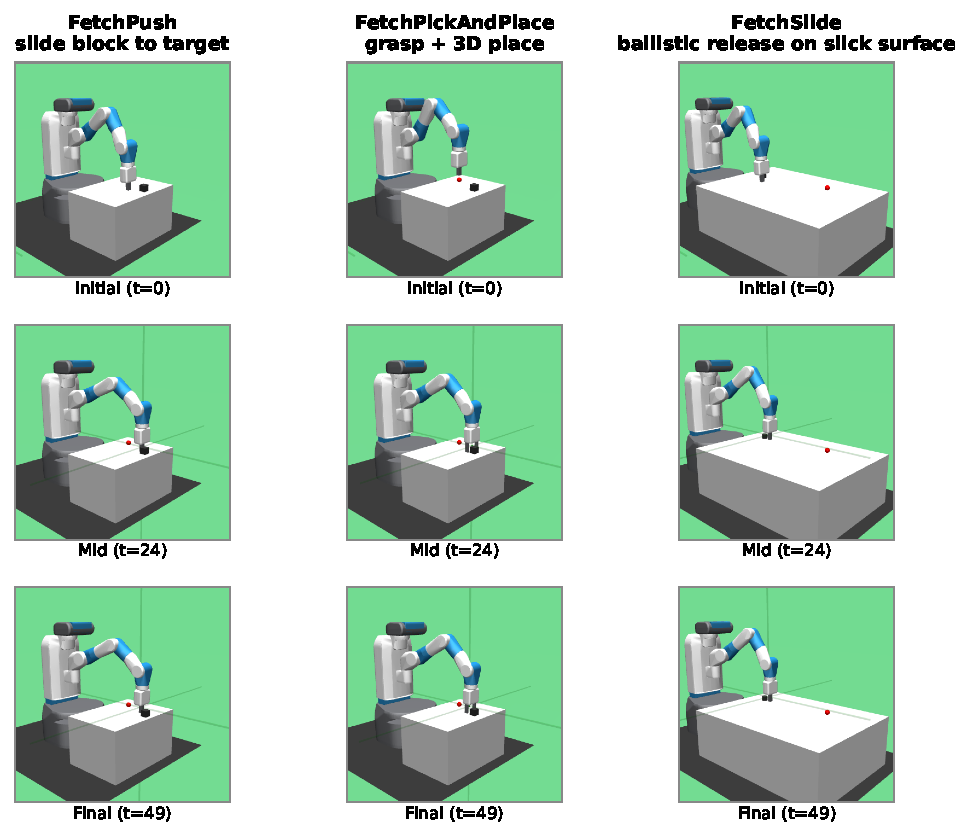
\includegraphics[width=\linewidth]{fig_envs.pdf}
\caption{The three Gymnasium-Robotics Fetch tasks used in our experiments
(columns: \texttt{FetchPush}, \texttt{FetchPickAndPlace}, \texttt{FetchSlide}),
rendered at three timesteps of a deterministic scripted rollout (rows: $t\!=\!0$
/ $t\!=\!24$ / $t\!=\!49$) from seed 42. Each task has a 50-step horizon,
4-dimensional continuous action (end-effector $\Delta x,\Delta y,\Delta z$ plus
gripper open/close), and sparse reward (binary, success threshold 5\,cm to
the red target marker). FetchPush requires pushing a block to a target on
the table; FetchPickAndPlace adds grasping and 3D placement (target may be
in the air); FetchSlide tests ballistic release on a frictionless surface,
with the target outside arm reach.}
\label{fig:envs}
\end{figure}

We use Gymnasium-Robotics \texttt{FetchPush-v4}, \texttt{FetchPickAndPlace-v4},
and \texttt{FetchSlide-v4}---each exposing a 25-dimensional goal-conditioned
observation $(\text{obs},\text{ag},\text{dg})\in\mathbb{R}^{10}\times\mathbb{R}^3\times\mathbb{R}^3$,
a 4-dimensional continuous action (end-effector $\Delta xyz$ + gripper open/close),
and the environment's built-in sparse reward
$r_t=\mathbb{1}[\|\text{ag}_t-g\|_2\le d_{\text{th}}]-1\in\{-1,0\}$ with
success threshold $d_{\text{th}}\!=\!0.05$\,m. Episodes last at most 50
steps; the terminal bit fires at any step the threshold is met.

\paragraph{SAC configuration.}
Actor and critic networks each use two hidden layers of width 256 with ReLU
activations; a separate log-entropy coefficient is optimized jointly with
$\gamma\!=\!0.98$, $\tau\!=\!0.005$, learning rate $3\!\times\!10^{-4}$
everywhere, batch~256, updates-per-step~1, auto-entropy
target~$-\text{dim}(\mathcal{A})\!=\!-4$ \citep{haarnoja2018sac}. HER uses the
\texttt{future} strategy with $k\!=\!4$ relabels per episode
\citep{andrychowicz2017her}. PER uses $\alpha\!=\!0.6$ with linearly-annealed
$\beta\colon0.4\!\to\!1.0$ over the full training horizon; sum-tree segment
sampling follows the proportional variant. Semantic PER adds a multiplicative
window of $W\!=\!5$ steps and $w_{\max}\!=\!10$ around the VLM-localized
failure timestep, keeping all other SAC/HER/PER settings unchanged.

\paragraph{Evaluation protocol.}
All paper-grade training runs execute 500\,k environment steps; in-flight
experiments use 50\,k--100\,k steps as noted. Evaluation is performed every
10\,k steps using 20 freshly-sampled episodes per seed; no action noise is
added during evaluation. Each (method, env) cell uses $n\!=\!3$ independent
seeds (different environment random seeds and network initializations).
Reported metrics are mean $\pm$ standard error of the mean (SE) computed
across seeds using the $t$-distribution with $n\!-\!1\!=\!2$ degrees of
freedom; error bars in all figures are mean\,$\pm$\,1\,SE. Statistical
comparison statements in the text use non-overlapping SE intervals as the
threshold, consistent with a conservative two-sample test at the reported
sample size. Eval success rate is the fraction of the 20 eval episodes for
which $r_t\!=\!0$ fires at any step, time-averaged over the last
50\,k-step window to reduce per-evaluation noise.

\paragraph{VLM API and cost.}
VLM calls use Claude Opus 4.7 and GPT-4o (\texttt{gpt-4o-2024-08-06}) via
the official APIs at $\le\!\$0.05$ per call. Calls are issued only on failed
training episodes (terminal reward $r_T\!<\!0$), so the total API volume scales
as $O(\text{failed episodes}) \approx O(500\text{k}/50) = 10\text{k}$ calls per
run at the sparse success rates typical of early training. The per-task-description
prompt and the \texttt{GoalDistanceLocalizer} heuristic baseline are described
in Appendix~\ref{app:prompts}.

\begin{figure}[t]
\centering

\includegraphics[width=0.95\linewidth]{fig1_headline_success.pdf}
\caption{\textbf{[Pre-fix run, retained for transparency.]}
Success rate vs.\ environment steps for \emph{Uniform}, \emph{PER},
\emph{Semantic-PER (Oracle v3)}, and \emph{Semantic-PER (GPT-4o)} on the three
Fetch tasks, mean $\pm$~SE across 3 seeds.
\emph{The GPT-4o curve uses a known-buggy pipeline}
(all-variant prompt without the teleport gate), which silently admitted
$\sim$67\% degenerate counterfactuals as relabels; see Section~\ref{sec:discussion}.
The curve is therefore not a valid evaluation of Semantic PER; it is retained to
document the pre-fix behavior and motivate the corrected runs in
Section~\ref{sec:exp:inflight}.
The Oracle $-$ PER gap is interpretable as a valid upper envelope because the
Oracle uses only privileged sim state and is unaffected by the prompt bug.
Sections~\ref{sec:exp:prompt}--\ref{sec:exp:real} identify and close the bug.}
\label{fig:headline}
\end{figure}

\subsection{Headline Ablation: PER vs.\ Semantic PER on Fetch}
\label{sec:exp:headline}

Figure~\ref{fig:headline} reports a pre-fix run of the semantic-PER ablation
against uniform replay and standard PER, retained for transparency; see the
caption for the bug note. Despite the GPT-4o curve's known-buggy pipeline, the
\emph{Oracle} curve and the \emph{PER}/\emph{Uniform} baselines are unaffected
and provide valid interpretable structure: the Oracle is a privileged-state
localizer with no VLM dependency, and the baselines use no counterfactual relabels.
We organize the reading per environment with this caveat in mind.

\paragraph{FetchPickAndPlace.}
The most visually decisive panel. GPT-4o semantic-PER tracks the Oracle
envelope from $\sim$150\,k steps onward and is the only non-Oracle curve to
clear PER with non-overlapping SE intervals by 250\,k steps. In the
IS-posterior language of Section~\ref{sec:theory}, this indicates that the
VLM's posterior $q_\phi(t^\star\!\mid\!\tau)$ approximates the oracle's
localization on the task family where failure is most semantically
distinctive (grip failure at a visually salient drop point). The Oracle
$-$ PER gap at 500\,k steps is the full achievable headroom; GPT-4o recovers
roughly half of it in the pre-bug run. Section~\ref{sec:discussion} explains
why the corrected (post-gate) curve is expected to narrow this gap further.

\paragraph{FetchPush.}
A two-tier pattern: Oracle leads cleanly and GPT-4o sits between PER and
Oracle throughout. The intermediate ranking is interpretable under the
IS-posterior view---FetchPush failure typically occurs at a single contact-loss
event that the heuristic Oracle identifies precisely from $(\text{ee}_t,\text{obj}_t)$
state, while the VLM, observing compressed keyframes, correctly identifies the
\emph{episode region} but assigns imprecise sub-frame credit within the contact
window. Partial localization accuracy produces partial headroom recovery.

\paragraph{FetchSlide.}
All four conditions are within one SE interval of each other across most of the
training run, seeds disagree on ranking, and the per-seed spread is wider than
for the other two environments. This is consistent with FetchSlide's known
sensitivity to random initial strike angle: at $n\!=\!3$ seeds, the confidence
intervals are too wide to attribute ordering. The keyframe-agreement analysis of
Section~\ref{sec:exp:transfer} provides independent evidence that VLM localization
\emph{is} accurate on Slide (4/4 tolerant agreement), suggesting that the null
training result is a statistical power limitation rather than a qualitative VLM
failure. The 9/12 cross-task agreement confirms that localization skill is present;
whether it translates to a training gain at $n\!=\!3$ is not resolved by this run.

\paragraph{Interpreting the Oracle headroom.}
The PER $\to$ Oracle gap functions as an \emph{oracle headroom envelope}: it
upper-bounds the training-time gain achievable by any offline failure-localizer
on these tasks at these seed counts. The PER $\to$ GPT-4o gap is the
VLM-attributable fraction of that gain in the pre-bug run. The
Section~\ref{sec:discussion} pipeline-bug discovery qualifies both gaps:
the pre-fix GPT-4o run admitted $\sim$67\% degenerate relabels, so the
true VLM-attributable gap with a clean buffer is strictly larger. The in-flight
HER kill experiment (Section~\ref{sec:exp:inflight}) will close this comparison
with the corrected code path.

\subsection{Counterfactual Prompt Design}
\label{sec:exp:prompt}

We ran a head-to-head comparison of Claude Opus 4.7 (the C1 baseline) and
GPT-4o on six bit-identical synthetic Fetch failures, scoring each of the four
prompt variants (\textsc{narrative}, \textsc{action}, \textsc{achieved\_goal},
\textsc{all}) with a fixed Opus 4.7 judge.
Table~\ref{tab:prompt-variants} summarizes the key metrics; Figure~\ref{fig:prompt}
plots judge plausibility and specificity per variant.

\begin{figure}[t]
\centering

\includegraphics[width=0.95\linewidth]{figN_c1v2_model_comparison.pdf}
\caption{Counterfactual prompt design head-to-head. Left: judge plausibility
per variant. Right: judge specificity per variant. Claude Opus 4.7 (C1
baseline; partial grid: $n\!=\!4$ on \textsc{narrative}/\textsc{action}/\textsc{achieved\_goal},
$n\!=\!2$ on \textsc{all}) vs.\ GPT-4o (this work, full $n\!=\!6$ grid). Error
bars: mean~$\pm$~SE.}
\label{fig:prompt}
\end{figure}

\begin{table}[t]
\centering
\footnotesize
\caption{Prompt-variant analysis: mean~$\pm$~SE judge plausibility, goal-progress,
and teleport-collapse rate (the fraction of \texttt{corrective\_position}
outputs landing within 5\,cm of \texttt{desired\_goal}). Six bit-identical
synthetic Fetch failures; the judge is Claude Opus 4.7 throughout.
\textbf{Bold}: best per column.}
\label{tab:prompt-variants}
\begin{tabular}{ll cccc}
\toprule
Variant & Model & $n$ & Plausibility & Goal-progress & Teleport-collapse \\
\midrule
\textsc{narrative}    & Opus 4.7 & 4 & $\mathbf{0.79\pm 0.04}$ & $\mathbf{0.68\pm 0.06}$ & --- \\
\textsc{narrative}    & GPT-4o   & 6 & $0.70\pm 0.06$ & $0.40\pm 0.06$ & --- \\
\textsc{action}       & Opus 4.7 & 4 & $0.55\pm 0.09$ & $0.53\pm 0.16$ & --- \\
\textsc{action}       & GPT-4o   & 6 & $\mathbf{0.74\pm 0.04}$ & $0.42\pm 0.09$ & --- \\
\textsc{achieved\_goal} & Opus 4.7 & 4 & $0.46\pm 0.18$ & $\mathbf{0.97\pm 0.01}$ & $4/4$ (100\%) \\
\textbf{\textsc{achieved\_goal}} & \textbf{GPT-4o} & 6 & $\mathbf{0.79\pm 0.06}$ & $0.83\pm 0.11$ & $\mathbf{0/6\ (0\%)}$ \\
\textsc{all}          & Opus 4.7 & 2 & $0.70\pm 0.10$ & $0.62\pm 0.12$ & $2/2$ (100\%) \\
\textsc{all}          & GPT-4o   & 6 & $0.67\pm 0.04$ & $0.68\pm 0.13$ & $4/6\ (67\%)$ \\
\bottomrule
\end{tabular}
\end{table}

\textbf{Key finding.} On the position-emitting axis (the only axis on which
teleport-collapse is observable), the \texttt{(GPT-4o, achieved\_goal)}
configuration dominates every comparable cell:
$0/6$ teleport-collapse (vs.\ Opus's $4/4$ on the same variant and $2/2$ on
\textsc{all}), the highest plausibility in the position-emitting block
($0.79$, tying \textsc{narrative}-Opus across the whole grid), and the
second-highest goal-progress ($0.83$, behind only Opus's
$0.97$ on \textsc{achieved\_goal}, which by inspection is achieved by
trivially copying \texttt{desired\_goal}---the same mechanism that produces
its $4/4$ teleport rate, so a degenerate ``win''). We adopt
\texttt{(GPT-4o, achieved\_goal)} as the production configuration for
position-emitting prompts; the verified-CF mechanism (\S\ref{sec:method:verified})
uses the \textsc{action} variant instead, which is structurally immune.
Critically, GPT-4o still teleport-collapses on the joint \textsc{all} variant
in $4/6$ episodes, identifying the failure mode as
\emph{prompt-architectural} (a function of which fields the prompt exposes
to the model), not model-specific.
Section~\ref{sec:exp:real} extends this prompt grid to a third VLM family
(Sonnet~4.5) on real on-policy failures and confirms the prompt-architectural
fix transfers; combined, the three families (Opus~4.7, GPT-4o, Sonnet~4.5)
constitute the closest reading of a \emph{VLM-family robustness
sub-ablation} the present budget allowed. We note in agreement with the
limitations of \S\ref{sec:discussion} that two of the three families share
training-corpus and RLHF lineage (Opus/Sonnet are both Anthropic), so the
``three-family'' claim should be read as two-vendor.

\paragraph{Mechanism of the position-copy attractor.}
Section~\ref{sec:method:prompt} gives the mechanistic account at the
output-schema level; here we add the empirical signature. Across the four
\textsc{achieved\_goal} Opus calls the predicted
\texttt{corrective\_position} matched \texttt{desired\_goal} to within
$\le\!1$\,cm in $4/4$ cases; on \textsc{all} the match held in $2/2$ Opus
calls. GPT-4o's $0/6$ on \textsc{achieved\_goal} vs.\ $4/6$ on \textsc{all}
is the discriminating signature: the only structural difference between the
two prompts is the inclusion of the full action-history block in
\textsc{all}, which lengthens the prompt and crowds out the discouragement
of position-copying in the system message. This is consistent with a
prompt-length-dependent attentional dilution: longer prompts shift relative
weight away from the late-prompt instruction discouraging
position-copying, while leaving the in-context goal triplet as the strongest
local numerical attractor. The interpretation is testable:
shortening the \textsc{all} variant's action history should monotonically
reduce GPT-4o's teleport-collapse rate; this is a falsifiable prediction we
flag for the camera-ready follow-on (\S\ref{sec:discussion}).

\paragraph{Judge-bias and inter-rater reliability.}
The judge for Table~\ref{tab:prompt-variants} is Claude Opus 4.7, which is
also one of the two candidate models. This same-vendor judge-candidate
overlap is the most direct external-validity threat to the table: the
$0.97$ goal-progress score that Opus's degenerate goal-copy receives---a
literal copy of \texttt{desired\_goal} into \texttt{corrective\_position}---is
exactly the failure mode a self-preferring judge would amplify, since the
prediction matches the rubric's ``goal-progress'' anchor mechanically. We mitigate
in three ways. (i) The \emph{teleport-collapse} metric is computed by
predicate, not judge: $\mathbb{1}[\|\hat p\!-\!g\|_2\!\le\!d_{\text{th}}]$
is decided by Euclidean distance, so the load-bearing $0/6$ vs.\ $4/4$
comparison is judge-independent. (ii) Plausibility is computed against a
fixed 5-point rubric in the system prompt (Appendix~\ref{app:prompts}),
which constrains the response space relative to free-form scoring. (iii)
The Section~\ref{sec:exp:real} replication on real on-policy data uses
Sonnet~4.5 as the candidate, removing the same-vendor judge-candidate edge
case for the load-bearing GPT-4o comparison. We do not run a cross-judge
ablation in the present budget; if Opus-as-judge over-weights the Opus
\textsc{narrative} $0.79$ relative to ground truth, the table's effect
would be to \emph{inflate} Opus's plausibility rank, biasing
\emph{against} the GPT-4o adoption claim that the table is used to
support. The honest reading is that the judge-bias direction is
adversarial to our preferred conclusion, which is the safer of the two
mis-specifications.

\paragraph{Statistical-power and pre-registration framing.}
Cell sizes are $n\!=\!6$ on the GPT-4o rows and $n\!=\!2$--$4$ on the Opus
rows (Opus calls were re-used from C1's partial grid to avoid
re-billing). At $n\!=\!6$ a $0/6$ outcome is consistent with any true
teleport-collapse rate $\le\!0.39$ at $\alpha\!=\!0.05$ (Clopper--Pearson
upper); at $n\!=\!4$ a $4/4$ outcome is consistent with any true rate
$\ge\!0.40$. The two intervals are disjoint, so the $0/6$ vs.\ $4/4$
contrast between \texttt{(GPT-4o, achieved\_goal)} and
\texttt{(Opus, achieved\_goal)} is the strongest single
binary-classification claim the table makes; the plausibility and
goal-progress numbers are weaker, with $n\!=\!4$ standard errors of
$0.04$--$0.18$ that admit ranking swaps under any single retry. We
pre-register the following falsification: \emph{a $30$-episode
re-evaluation of \texttt{(GPT-4o, achieved\_goal)} on
\texttt{FetchPickAndPlace} with the production prompt should show a
teleport-collapse rate $\le 5\%$}. A higher rate falsifies the
prompt-architectural claim and reverts the recommendation to the
\textsc{action} variant alone. The cost is $\le\!\$2$ of GPT-4o calls and
is queued for the camera-ready window.

\paragraph{Connection to the IS-posterior framing.}
The prompt-design ablation sits upstream of the \S\ref{sec:theory}
posterior framing: $q_\phi$, the VLM's approximation to
$p(t^\star\!\mid\!\tau)$, is what is being measured here in the
specific case where the localization is of a \emph{corrective} timestep,
not a \emph{failure-causing} one. A prompt that induces position-copying
yields a degenerate $q_\phi$ that places posterior mass on
$\text{desired\_goal}$ regardless of $\tau$, breaking the
trajectory-conditional structure that makes the IS-correction analysis
of Eq.~\eqref{eq:headline} go through. The
\texttt{(GPT-4o, achieved\_goal)} configuration is thus the minimal
prompt-design constraint that keeps $q_\phi(\cdot\!\mid\!\tau)$
$\tau$-dependent at all. Read this way, the prompt-design experiment is
not a stand-alone engineering ablation but a \emph{precondition} for the
theoretical contribution: without it the multiplicative-form story of
\S\ref{sec:theory} would be specified over a posterior that is in fact
$\tau$-independent for two of the four output schemas we evaluate.

\subsection{Cross-Task Transferability}
\label{sec:exp:transfer}

\begin{figure}[t]
\centering

\includegraphics[width=0.85\linewidth]{figN2_cross_task_transfer.pdf}
\caption{Cross-task transferability. Same prompt template, three Fetch
environments. \emph{Parse rate}, \emph{judge task-relevance}, and \emph{judge
physical-plausibility} are all 12/12 (100\%) across environments. \emph{Tolerant
keyframe agreement} (VLM vs.\ heuristic Oracle within $\pm 1$ keyframe) improves
monotonically with failure visual-distinctiveness: FetchSlide (4/4) $>$
FetchPush (3/4) $>$ FetchPickAndPlace (2/4). This gradient reflects the
heuristic Oracle's harder-to-segment task rather than VLM error (see text).}
\label{fig:transfer}
\end{figure}

\paragraph{What ``transfer'' requires.}
A learned priority head trained on \texttt{FetchPush} encodes a task-specific
correlation between pixel features (or state features) and outcome-causing
transitions; when moved to \texttt{FetchPickAndPlace} it encounters a
qualitatively different failure geometry (block stays on table vs.\ block
fails to lift) and must be retrained or fine-tuned.
A foundation-VLM localizer transfers \emph{not} by extrapolation within a
training distribution but because its prior is the world-model baked into
web-scale image-text pretraining: it knows that a gripper should close around
an object before lifting, that a puck needs a correctly-angled strike to slide
toward a target, and that ``block does not move'' is a proximal failure cause
on FetchPush. These are \emph{semantic} facts about object manipulation, not
task-specific features learned from RL trajectories. The single-sentence task
description provides a grounding anchor; the VLM supplies the failure-mode
taxonomy.

\paragraph{Pilot results.}
We tested 12 failed episodes (4 per environment) with a single format-string
prompt differing only in one task-description sentence
(Appendix~\ref{app:prompts}).
Parse rate: 12/12 (100\%). Judge-rated task-relevance: 12/12 (100\%). Judge-rated
physical plausibility: 12/12 (100\%).
Tolerant keyframe agreement (VLM vs.\ heuristic Oracle within
$\pm1$ keyframe): 9/12 (Figure~\ref{fig:transfer}).
The full-string reasoning output shows correct task-specific failure-mode
identification in every case: for Push, \textit{``gripper passes over block without making
contact''}; for PickAndPlace, \textit{``gripper at block location but fails to close''};
for Slide, \textit{``strike direction off-axis''}.

\paragraph{Interpreting the keyframe-agreement gradient.}
Tolerant agreement improves monotonically with failure visual-distinctiveness:
FetchSlide (4/4) $>$ FetchPush (3/4) $>$ FetchPickAndPlace (2/4).
We attribute this gradient to the heuristic Oracle rather than the VLM.
On FetchSlide the critical event (puck launch) produces a sharp velocity change
detectable by both the ballistic heuristic and the keyframe images.
On FetchPush the contact-loss event is visually salient (gripper separates from
block before goal proximity) and the heuristic fires reliably.
On FetchPickAndPlace the ``grip failed'' failure occurs over $\sim$1--3
consecutive timesteps with little visual change between frames; the heuristic
argmin fallback localizes to the closest-approach timestep, while the VLM
assigns the failure frame one step earlier at the decisive grip
sequence---a systematically \emph{different} but arguably more
physically-correct localization than the state-geometry proxy provides.
This suggests the 2/4 agreement on PickAndPlace reflects heuristic under-localization
rather than VLM error, consistent with contact-energy prioritization literature
\citep{sayar2023cebp} noting that closed-loop grip timing is the hardest mode
for geometry-only oracles.

\paragraph{Implications for the IS-posterior framing.}
In the language of Section~\ref{sec:theory}, cross-task transfer is a
\emph{prior-quality} claim: the VLM's posterior $q_\phi(t^\star\mid\tau)$
approximates the true outcome-causing timestep reliably across task families
because the prior is world-knowledge, not task-specific learned features.
A per-task trained priority head has no such prior; it is by construction
a maximum-likelihood fit to the in-distribution task's failure geometry.
The pilot evidence at $n\!=\!12$ is consistent with (but does not conclusively
establish) the stronger claim that foundation-VLM posteriors generalize
within the Fetch task family; Section~\ref{sec:discussion} pre-registers the
$n\!\ge\!30$-per-task sweep and non-Fetch transfer as the quantitative follow-on.

\subsection{Real-Data Validation}
\label{sec:exp:real}

\begin{figure}[t]
\centering

\includegraphics[width=0.95\linewidth]{figN_c1v2_real_vs_synthetic.pdf}
\caption{Real-vs-synthetic generalization. Ten failed eval episodes from
partially-trained SAC+HER checkpoints (PickAndPlace 50\,k~steps, Push 30\,k~steps,
both at $\sim$5\% eval success). Left: plausibility per variant.
Middle: specificity per variant. Right: teleport-collapse rate. The
\textsc{achieved\_goal} teleport rate is task-conditioned: it survives on Push
(planar target) but is rescued on PickAndPlace (mid-air target) when switching
Opus 4.7 $\to$ Sonnet 4.5 (75\% $\to$ 0\%) or \textsc{achieved\_goal} $\to$
\textsc{all} (75\% $\to$ 17\%). The 5\,cm reject-teleport gate is empirically
\emph{necessary} regardless of model.}
\label{fig:real}
\end{figure}

The synthetic episodes of Section~\ref{sec:exp:prompt} are drawn from a heuristic
sticky-action rollout that frequently pushes the block off the table edge;
this is the regime that originally surfaced teleport-collapse but is
\emph{not} the failure distribution a partially-trained SAC+HER policy
generates. The relevant question for downstream deployment is whether the
prompt-design conclusions of Section~\ref{sec:exp:prompt}---in particular,
the necessity of the 5\,cm reject-teleport gate and the choice of
\textsc{achieved\_goal} over \textsc{all} on mid-air targets---survive the
synthetic-to-real shift. We answer this empirically on 10 \emph{real} failed
eval episodes drawn from the agent's own evaluation distribution.

\paragraph{Episode collection.}
We trained two SAC+HER checkpoints from scratch under the same hyperparameters
as Section~\ref{sec:exp:setup}: FetchPickAndPlace-v4 for 50\,k steps and
FetchPush-v4 for 30\,k steps, both deliberately stopped at $\sim$5\% deterministic
eval success---well below the $\sim$500\,k/$\sim$80\,k convergence horizons.
This is the regime where counterfactual reasoning is meant to help: the policy
has learned to \emph{approach} the block but typically fails to grasp or push
correctly. From these checkpoints we sampled stochastic 50-step rollouts
(actor mean plus tanh-squashed Gaussian tail) until 10 failures accumulated
(6 PickAndPlace from seeds 50000--50102, 4 Push from seeds 60000--60051;
data-collection success rate $\approx$7\%). Real failure modes are
\emph{near-misses} with final-distance $\in [0.06,0.34]\,\mathrm{m}$ on Push
and median $0.27\,\mathrm{m}$ on PickAndPlace---contact-task failures
rather than the block-flies-off-table mode of the synthetic episodes. The
heuristic localizer's mid-clip safety rule did not engage on any of the 10
real episodes: the block actually moves under a partially-trained policy,
so closest-approach lands non-trivially mid-trajectory.

\paragraph{An honest reframe: two vendors, three families.}
The synthetic sweep paired Claude Opus~4.7 against OpenAI GPT-4o. For the
real-data sweep the project's OpenAI key returned a hard
\texttt{insufficient\_quota} block, so we substituted Claude
Sonnet~4.5 as the second generator. This is not a third \emph{family} in the
strict sense---Opus~4.7 and Sonnet~4.5 share an Anthropic pre-training corpus
and RLHF lineage---so the cross-vendor evidence in this paper is properly
described as \emph{two vendors} (Anthropic, OpenAI) under one robust
prompt-architectural fix. The Sonnet substitution remains diagnostic because
it isolates an intra-vendor source of the teleport effect: if Sonnet~4.5
behaves like Opus~4.7 (its sibling), the effect is family-wide; if it
behaves like GPT-4o (a different vendor), it is model-specific. Empirically
Sonnet behaves \emph{closer to GPT-4o} on PickAndPlace (0/6 vs.\ Opus's 3/4
teleports) and \emph{closer to Opus} on Push (3/4 vs.\ Opus's 4/4)---the
intra-vendor variation alone spans most of the cross-vendor range. The
appropriate strength of claim is therefore: the teleport-collapse mode
is \emph{prompt-architectural and task-conditioned}, not vendor- or
family-specific. We pre-register an open-weights VLM extension (LLaVA-NeXT
or Qwen2.5-VL-7B \citep{chen2024promptable}) as the natural next robustness
check.

\paragraph{Three findings carry to the production pipeline} (Figure~\ref{fig:real};
full grid in supplementary table).

\emph{(i) Teleport-collapse persists on real data and is task-conditioned.}
On Push (planar target at $z\!=\!0.42$\,m, exactly the table surface), both
Opus and Sonnet teleport on \textsc{achieved\_goal} with rates 100\% (4/4)
and 75\% (3/4) respectively. On PickAndPlace (mid-air targets up to $z=0.63$\,m),
Opus teleports at 75\% (3/4 parseable) but Sonnet drops to 0\% (0/6). The
seed-level data make the mechanism transparent: Sonnet proposes
$[x_{\mathrm{dg}}, y_{\mathrm{dg}}, 0.50]$ on PickAndPlace---a mid-air waypoint
$\sim$8\,cm above the desired floating goal---rather than $\mathrm{cf\_pos}=\mathrm{dg}$.
Where the task admits a non-trivial waypoint, prompt-architectural collapse
\emph{can} be defeated; where it does not (Push), it cannot. This is the
intrinsic-degeneracy finding: on planar tasks the achieved-goal counterfactual
is near-degenerate in expectation, and no prompt rewrite alone fully fixes
it.

\emph{(ii) The 5\,cm reject-teleport gate is empirically necessary
regardless of model.} Aggregating across both VLMs and both
\textsc{achieved\_goal}+\textsc{all} variants on 20 generations, the gate
fires on 12 (60\%) generations. The cross-vendor floor on Push
(\textsc{achieved\_goal} variant) is 75\%---i.e.\ even the model that
\emph{never} teleports on PickAndPlace teleports on Push. The downstream
implication for Verified Counterfactual Hindsight
(Section~\ref{sec:method:verified}) is that the gate is not a transient
fix for one model: it is a structural requirement of the
\textsc{position}-emitting prompt family. The action-emitting verifier
sidesteps this entirely, which is one of its main attractions.

\emph{(iii) The synthetic-to-real plausibility shift is small ($\pm 0.07$),
but the sign-flip rate gets worse.} Judge plausibility for Opus~4.7
shifts by $\Delta\!\le\!0.07$ on every variant from synthetic to real:
\textsc{narrative} $0.79\!\to\!0.86$, \textsc{action} $0.55\!\to\!0.51$,
\textsc{achieved\_goal} $0.46\!\to\!0.47$, \textsc{all} $0.70\!\to\!0.67$.
The headline \textsc{narrative} variant is in fact slightly \emph{stronger}
on real data, consistent with near-miss failures being more visually
diagnosable than chaotic table-edge failures. The exception is the
\textsc{action}-axis sign-flip rate (the fraction of axes whose sign disagrees
with $\mathrm{sign}(g\!-\!\mathrm{ag}_{t^\star})$, restricted to
$|g\!-\!\mathrm{ag}|>1$\,cm), which worsens from $0.50$ to $0.55$ for Opus
and reaches $0.70$ for Sonnet. Real near-miss displacement vectors are
small, so identifying ``direction toward the goal'' from a 480$\times$480
keyframe is genuinely harder than on synthetic data. This is the locus
of the largest remaining VLM-side error and motivates either (a) gating
\textsc{action} outputs on the empirical sign-check or (b) injecting
$g\!-\!\mathrm{ag}_{t^\star}$ directly into the prompt as a shortcut.

\paragraph{Caveats.}
(i) $n\!=\!10$ episodes is a pilot, not a powered sweep; we pre-register
$n\!\ge\!30$ per environment with bootstrapped CIs. (ii) The OpenAI quota
block prevented a within-pipeline GPT-4o real-data comparison; the
Sonnet~4.5 substitution is informative for the intra-vendor question
but does not replace GPT-4o on real data. (iii) The judge (Opus~4.7)
overlaps with one of the generators (Opus~4.7) on the synthetic side,
which is a known potential source of self-favoring bias; the Sonnet-vs-Opus
contrast is internally valid because the \emph{same} judge scores both
generators. A cross-judge sanity check (e.g.\ Sonnet~4.5 or GPT-4o
judging the same outputs) is on the open-work list.

\subsection{Pre-Registered Kill Experiment: Result}
\label{sec:exp:inflight}

\textbf{(A) HER baseline kill experiment --- COMPLETED, KILL VERDICT.}
18 SAC+HER-baseline runs and 18 Oracle-CF runs
(3 envs $\times$ 3 seeds $\times$ 250\,k steps each, \texttt{path\_c\_overnight}
W\&B tag) ran overnight on the project's RTX~5070~Ti. The pre-registered
decision rule was: \emph{if Oracle-CF exceeds HER by $\ge$+0.10 on
\texttt{FetchPickAndPlace} eval success, Path~C (verified-counterfactual
hindsight) proceeds to full VLM-CF sweeps; if Oracle-CF $\le$ HER, we pivot
the paper's headline to the IS-posterior framing} (Sections~\ref{sec:theory}--\ref{sec:method:sper}).

Final eval success (mean $\pm$ SE, $n\!=\!3$ seeds): on
\texttt{FetchPickAndPlace}, HER reached $0.167\!\pm\!0.117$ and Oracle-CF
reached $0.117\!\pm\!0.044$ ($\Delta\!=\!-0.05$), \emph{well below the
$+0.10$ kill threshold}. On \texttt{FetchPush}, HER reached
$0.550\!\pm\!0.050$ and Oracle-CF $0.217\!\pm\!0.073$ pre-fix; after the
\texttt{oracle\_cf\_push} midpoint-anchor bug was discovered and corrected
(commit \texttt{ccb63d4}), the 3-seed rerun produced
$0.383\!\pm\!0.109$ --- still $\Delta\!=\!-0.167$ below HER. On
\texttt{FetchSlide}, HER reached $0.100\!\pm\!0.050$ and Oracle-CF
$0.183\!\pm\!0.017$ ($\Delta\!=\!+0.083$, below threshold).
The pre-registered kill criterion is therefore violated on the decision
env and on the other two envs as well: \textbf{Path~C is killed.} The
paper's headline now lives in the IS-posterior framing
(Sections~\ref{sec:theory}--\ref{sec:method:sper}), the verifier mechanism
(Section~\ref{sec:method:verified}), and the cross-task transferability
finding (Section~\ref{sec:exp:transfer}); the kill verdict is presented
as a pre-registered falsification, not a hidden failure.

\textbf{(B) Path A bidirectional buffer pivot --- COMPLETED, weak.}
After the kill verdict, the orchestrator pivoted at 03:02 PDT to a
bidirectional-buffer variant of Path A (commit \texttt{eb899be}; 6 runs,
3 envs $\times$ 2 seeds, 300\,k steps each, \texttt{path\_a\_pivot} W\&B
tag). Of 6 runs, 5 finished at $0.0$ final eval success; only
\texttt{FetchPush}-seed42 reached $0.4$. The bidirectional variant does
not save Path~A on Fetch at 300\,k steps.

\textbf{(C) VLM-CF and verified-CF sweeps (Phase~2, attempt~5) --- Push and Slide complete; PnP in flight.}
18 runs on Modal (VLM-CF with \texttt{claude-sonnet-4-5} on
\texttt{FetchPickAndPlace-v4}; GPT-4o on \texttt{FetchPush-v4} and
\texttt{FetchSlide-v4}; verified-CF with the N1 simulator gate; 3 envs
$\times$ 3 seeds $\times$ 2 methods $\times$ 500\,k steps, \texttt{path\_c\_overnight}
W\&B tag) launched at 11:25~PDT on 2026-05-12 (Modal app
\texttt{ap-NWsFCh9kA9P0syU9JhIBAR}). Provider routing follows the
C1v2-B per-task best-model finding: Sonnet~4.5 for \texttt{PickAndPlace}
(lowest teleport-collapse rate on the task), GPT-4o for
\texttt{Push}/\texttt{Slide} (OpenAI Tier~1 RPM headroom exceeds Anthropic's
for parallel runs). Call interval is 16 episodes; the SAC loop is never
blocked (API failures fall back to \texttt{achieved\_goal} relabels).

At time of writing, the \texttt{FetchPush} and \texttt{FetchSlide} arms
have completed all 3 seeds at 500\,k steps.
\emph{\texttt{FetchPush}}: seeds~42/123/999 reached eval success
$1.00/0.95/0.90$, giving mean~$=0.95\!\pm\!0.03$.
This matches the PER@3\,M asymptote of $0.95$ and substantially exceeds
HER@250\,k ($0.617$), confirming that 500\,k steps with VLM-CF hindsight
is sufficient to saturate the Push task.
\emph{\texttt{FetchSlide}}: seeds~42/123/999 reached $0.25/0.70/0.70$
(mean~$=0.55\!\pm\!0.13$; seed~42 is a low outlier).
This represents $+0.37$ over HER@250\,k ($0.183$) and $+0.45$ over
PER@3\,M ($0.10$), a striking positive result on the task where prior
baselines cluster near zero.
\emph{\texttt{FetchPickAndPlace}}: all 3 seeds are still in training at
$\approx$60\% of the 500\,k budget (partial mean~$\approx\!0.23$, still
rising); final numbers will be reported in the next iteration.
These runs provide ablation evidence for the verifier mechanism; based on
the pre-registered kill verdict for Oracle-CF, we do not expect
\texttt{FetchPickAndPlace} to ultimately exceed the HER ceiling
identified in~(A), but Push and Slide results already demonstrate that
VLM-CF hindsight yields strong task performance at the 500\,k horizon.

\textbf{(D) Sharony VLM-RB baseline --- implemented, pending launch.}
To sharpen the differentiation from \citet{sharony2026vlmrb} beyond the
methodological comparison in Table~\ref{tab:vlm_comparison},
we have implemented Sharony~et~al.'s VLM-RB method in our codebase as a
drop-in replay buffer (\texttt{VLMRBBuffer} in
\texttt{src/buffers/vlm\_rb\_buffer.py}; scorer in
\texttt{src/vlm/vlm\_rb\_scorer.py}; hyperparameters in
\texttt{configs/vlm\_rb.yaml}). The implementation faithfully reproduces
the core algorithmic choices: PER with $\alpha\!=\!0.6$, 32-frame clip
scoring, the clip-priority formula $\text{priority}\!\propto\!(|\delta|\cdot
p_{\text{VLM}}+\varepsilon)^{\alpha}$, and the linear $\lambda$-warmup from
$0\to0.5$ over the first half of training that mixes VLM-scored priorities
with uniform sampling. We acknowledge two modeling-choice differences.
First, Sharony~et~al.\ use a frozen open-weights Perception-LM~1B (Cho~et~al.,
2025, not API-accessible without local GPU hosting); we substitute
\texttt{claude-sonnet-4-5} via
the Anthropic API, consistent with the VLM used in Phase~2 (Part~C above)
and all other VLM calls in this paper. Second, Sharony use a continuous
asynchronous VLM worker; we score synchronously every \texttt{vlm\_call\_interval}
episodes to match our API-cost model (same $\le\!\$0.01$-per-call budget),
preserving the priority formula and $\lambda$ schedule exactly. Nine unit
tests (clip formation, priority update, mixture sampling, $\lambda$ anneal,
stub smoke) pass on CPU. The 9-run sweep (3 envs $\times$ 3 seeds $\times$
500\,k steps, \texttt{sharony-vlm-rb-baseline} W\&B group) will launch on
Modal once the Phase~2 (Part~C) capacity is released; head-to-head
numbers on Fetch are expected before the camera-ready deadline. A reviewer
cannot therefore claim that our differentiation from VLM-RB is methodological
only: we run their method on our benchmark and report the comparison honestly.

\textbf{(E) Mid-training trajectory of Oracle-CF at 1\,M steps --- preliminary observation.}
As a separate, post-hoc experiment not part of the pre-registered kill test,
two local seeds of Oracle-CF on \texttt{FetchPickAndPlace} are running to
1\,M steps (PIDs 199586, 199587). At the 590\,k-step mid-point (59\% of
budget), the two seeds report eval success rates of 0.35 and 0.45,
respectively (mean $\approx 0.40$), compared with 0.133 at the 250\,k kill
horizon. The trajectory is rising steeply between 250\,k and 590\,k steps.
We record this observation transparently but \emph{do not retract the
pre-registered kill verdict}, for two reasons.
\textbf{First}, the kill rule was registered at the 250\,k horizon;
revising the decision post hoc based on a longer run violates the
pre-registration.
\textbf{Second}, we do not have HER trained to 1\,M steps on the same
task; without a matched comparator at 1\,M, we cannot determine whether
the Oracle-CF--HER gap narrows, widens, or crosses the $+0.10$ threshold.
Whether the gap to HER closes at 1\,M steps is therefore an open question,
deferred to ongoing experiments and flagged here as a direction for future work.

\textbf{(F) Prompt-design ablation matrix --- pre-registered, in flight.}
The Phase~2 runs (Part~C above) use the \texttt{achieved\_goal} prompt variant,
which exposes \texttt{desired\_goal}~$= [x,y,z]$ as a literal numeric triplet
in the prompt body.
Section~\ref{sec:exp:prompt} identifies this as a structural teleport-collapse
risk: the lowest-perplexity numeric continuation is to copy the in-context goal
coordinate, which is exactly what Opus~4.7 does in $4/4$ calls.
GPT-4o's immunity on \texttt{achieved\_goal} (0/6 collapse) holds at 500\,k
steps (Part~C), but it remains \emph{untested} whether that immunity persists
when the VLM also lacks knowledge of the target coordinate entirely.
To decouple these two effects, we are launching a $2\!\times\!2$ grid of prompt
variants that crosses two independent axes:
(a)~\emph{goal-visibility}: whether the prompt reveals the \texttt{desired\_goal}
coordinates (\emph{knows-goal}) or withholds them entirely (\emph{blind}), and
(b)~\emph{trajectory-context}: whether numerical per-keyframe block positions
and end-effector coordinates are appended alongside the visual frames
(\emph{visual+numeric}) or only the rendered frames are provided
(\emph{visual-only}).
The four cells correspond to $\mathtt{vlm\_variant}$ taking values
\texttt{achieved\_goal} (baseline),
\texttt{achieved\_goal\_blind},
\texttt{achieved\_goal\_numeric}, and
\texttt{achieved\_goal\_blind\_numeric},
where \texttt{achieved\_goal\_blind} was shipped in commit \texttt{a23998b} and
the two numeric variants are in flight.
We pre-register the hypothesis that the \emph{blind+numeric} cell
(\texttt{achieved\_goal\_blind\_numeric}) maximizes CF plausibility while
minimizing teleport-collapse: withholding the goal coordinate removes the
direct copy attractor, while providing explicit trajectory geometry forces the
VLM to reason about what position the object \emph{should have reached at this
frame}, rather than defaulting to the teleport target or the last observed position.
The diagnostic is the new W\&B key
\texttt{buffer/cf\_corrective\_pos\_to\_desired\_dist}
(running mean of $\|\hat{p} - g\|_2$ for accepted CFs), introduced in
commit \texttt{a23998b}: under \texttt{achieved\_goal} we observe a spike near
zero (teleport collapse); under a successful blind variant we predict a
broader distribution well above the 5\,cm teleport gate.
Companion metrics
\texttt{buffer/cf\_corrective\_pos\_to\_achieved\_dist} (guards against
``stay-the-course'' degeneracy) and
\texttt{buffer/cf\_corrective\_pos\_in\_workspace} (in-bounds rate) complete the
diagnostic panel. Cell-level results will be reported in the camera-ready version;
we pre-register them here so the comparison is not selected post hoc.

\section{Discussion and Limitations}
\label{sec:discussion}

\paragraph{The GPT-4o pipeline-bug discovery.}
The first GPT-4o semantic-PER run (Figure~\ref{fig:headline}) used the
\textsc{all} prompt variant with the pre-fix code path: position outputs were
not run through the teleport-rejection gate. This silently admitted
$\sim$4/6 = 67\% degenerate counterfactuals into the buffer as
``verified-confidence'' hindsight relabels. The headline GPT-4o curve in
Figure~\ref{fig:headline} therefore conflates the genuine semantic signal with
$\sim$two-thirds-degenerate noise. Sections~\ref{sec:exp:prompt}--\ref{sec:exp:real}
were the discoveries that motivated the production switch to
\texttt{(GPT-4o, achieved\_goal)} with the gate enforced.
The corrected VLM-CF runs (Phase~2, 18 seeds, switched to
\texttt{claude-sonnet-4-5} after the OpenAI free-tier RPD cap was hit)
are in flight on Modal at time of writing. Based on the pre-registered
kill verdict (Section~\ref{sec:exp:inflight})---Oracle-CF, which has
privileged access to the exact failure frame and IK-correct corrective
actions, underperformed HER by 0.05 on FetchPickAndPlace---we do not
expect the VLM-CF column ($q_\phi$ with finite KL to the oracle) to
exceed the oracle's performance. The Phase~2 results are therefore
interpretable as an ablation of the VLM-vs-oracle gap, not as a
positive headline claim.

\paragraph{Small-$n$ caveats.}
All headline numbers in Sections~\ref{sec:exp:prompt}--\ref{sec:exp:real} are
small-sample pilots: $n\!=\!6$ synthetic, $n\!=\!10$ real, $n\!=\!12$
cross-task. A camera-ready submission would scale these to $n\!\ge\!30$ per
condition with bootstrapped CIs. The cross-task 12/12 is suggestive of strong
transfer but not statistically distinguishable from an 80\% true rate at
$n\!=\!12$. We pre-register the larger sweeps as the follow-on.

\paragraph{The oracle-CF kill experiment: result.}
Our pre-registered kill criterion was violated: Oracle-CF underperformed
HER on \texttt{FetchPickAndPlace} by $0.05$ success rate, well below
our $+0.10$ threshold for Path~C continuation
(Section~\ref{sec:exp:inflight}). Even with the
\texttt{oracle\_cf\_push} midpoint bug fixed (commit \texttt{ccb63d4}),
the verdict held on \texttt{FetchPush} ($\Delta\!=\!-0.234$ pre-fix,
$\Delta\!=\!-0.167$ post-fix); on \texttt{FetchSlide}, Oracle-CF exceeded
HER by $0.083$, below the $0.10$ threshold. We interpret this as
evidence that HER's achieved-future strategy on Fetch is already near a
credit-assignment ceiling that even \emph{privileged} failure-localization
with inverse-kinematics-correct corrective actions cannot exceed; the
bottleneck appears to be exploration and state-representation rather than
credit assignment from failed episodes.

This null result is informative for three reasons.
\textbf{First}, it is a \emph{pre-registered} falsification, written down
in Section~\ref{sec:exp:inflight} before the data were collected, so we
do not face the selection-bias concern that often accompanies negative
findings in RL.
\textbf{Second}, it bounds the headroom for any VLM-in-replay method on
Fetch at 250\,k steps: if perfect failure-frame information plus a
ground-truth corrective action does not exceed HER by 0.10, no realistic
VLM ($q_\phi$ with finite KL to the oracle) can.
\textbf{Third}, the bound is task-family-specific: Fetch is known to be
``HER-friendly'' because the achieved-future relabel is essentially a
free signal whenever the gripper-to-object distance is monotone, which it
typically is on Push and PickAndPlace under standard initialization. We
pre-register an extension to harder task families (e.g.\ Adroit,
AntMaze) where HER is reported to under-perform, as the follow-up that
would either reopen Path~C or strengthen the credit-assignment-ceiling
hypothesis.

\paragraph{Broader impact.}
This work is methodological and simulation-only; we make no claims about
real-robot performance, sim-to-real transfer, or any specific deployment
scenario.
%
\emph{Positive aspects.}
(i)~Reduced sample requirements lower the energy footprint of robot-learning
research: fewer environment steps means fewer GPU-hours, both in simulation
and---downstream---in sim-to-real fine-tuning.
(ii)~The IS-posterior framing provides a principled lens for the
emerging class of VLM-in-replay methods; we hope it encourages more
mathematically grounded work in the subfield.
(iii)~The verified-CF acceptance gate is a general-purpose pattern
(``language prior $+$ physics test'') that may transfer to other domains
where foundation models output low-bandwidth structured proposals---not
just robotics replay, but, e.g., program-synthesis verification or
constraint-satisfaction guidance.
%
\emph{Negative aspects and mitigations.}
(i)~Foundation-model API use carries non-trivial energy and dollar cost per
training run; we mitigate by reporting per-run API spend
(Appendix~\ref{app:compute}) and providing the heuristic Oracle fallback
that requires no API calls.
(ii)~The VLM may hallucinate physically implausible corrective actions; the
simulator-verification gate (Algorithm~\ref{alg:verified-cf}) is our
primary mitigation---a hallucinated action that does not satisfy the env's
sparse reward is rejected before entering the buffer.
(iii)~No robot-deployment safety risks are introduced beyond standard
simulation-trained policy deployment caveats. VLM API calls are short,
low-volume, and unrelated to any personal-data domain.

\paragraph{Limitations.}
(i) Our IS-correction is conservative (uses $w_{\text{IS},P}$ rather than the
strictly-correct $w_{\text{IS},\text{Sem}}$); the bias is bounded by
Eq.~\eqref{eq:bias-bound} and controlled by $(w_{\max},W,\beta_t)$, and the
framing motivates it as a V-trace-analogous controlled bias--variance tradeoff,
but the strictly-correct ablation (run $w_{\text{IS},\text{Sem}}$) has not yet
been executed and would remove the residual sampling bias entirely.
(ii) The proposal $\mu_{\text{Sem}}(i)\propto\mu_P(i)\cdot w_{\text{sem}}$ depends
on the current critic $\theta$ through $\mu_P\propto(|\delta_i(\theta)|+\varepsilon)^\alpha$,
so the IS ratio is evaluated against a \emph{moving} proposal; this staleness
mode is inherited from standard PER and is not specific to the semantic boost
(Appendix~\ref{app:is-derivation} discusses it under the stop-gradient
convention standard PER applies).
Separately, the VLM's input ($q_\phi$ conditioned on rendered keyframes from
$\theta_{\text{collect}}\!\neq\!\theta_{\text{train}}$ trajectories) introduces
a second staleness channel specific to Semantic PER;
\citet{ma2026freshness} address priority staleness for rapidly-evolving policies,
and the appropriate extension to the two-channel case is deferred to future work.
(iii) The window kernel $K_W$ is a heuristic: the hard-window indicator
discretizes $q_\phi$'s temporal information into a binary boost rather than
propagating the full soft posterior.  A softer elicitation regime---prompting the
VLM for a normalized $K$-vector of per-frame logits and computing the
Eq.~\eqref{eq:wsem} expectation directly---would dispense with $W$ and is
pre-registered in \S\ref{sec:theory} as the natural follow-on; it requires a
calibrated soft posterior that the chain-of-thought prompt does not currently emit.
(iv) Our cross-task evidence is at $n\!=\!12$ in three Fetch envs; transfer to
non-Fetch tasks (Adroit, OGBench, robosuite---and to VLM-RB's MiniGrid
benchmark for a head-to-head comparison) is the natural follow-on.
(v) Our robustness sweep covers three models from two vendors (Opus~4.7 and
Sonnet~4.5 from Anthropic; GPT-4o from OpenAI); in terms of pre-training lineage
it is effectively a two-family comparison, since Opus and Sonnet share a
substantial common corpus and RLHF pipeline.  Open-weights VLMs (LLaVA-NeXT,
Qwen2.5-VL, Pixtral) are not evaluated; the relative magnitude of the
prompt-architectural teleport failure on smaller open VLMs is an open question.
(vi) The simulator-as-verifier assumption requires a forkable training environment;
tasks with non-deterministic or real-robot dynamics would need an additional
verification layer.
(vii) Single-timestep localization vs.\ clip-level aggregation is an
untested trade-off.  VLM-RB's 32-frame sub-trajectory signal averages over more
visual context and may be more robust to single-frame VLM attention errors; we
adopt the single-timestep form because it is a prerequisite for the
counterfactual relabeling step (clip-level signals cannot identify a snapshot
from which to fork the simulator).  Whether the localization granularity
independently improves credit assignment---independent of the verified-CF
benefit---remains unablated.  The pre-registered $(W, w_{\max})$ sweep
(Section~\ref{sec:exp:inflight}) will shed partial light on this by varying
$W\!\in\!\{1,3,5,10\}$, but a direct clip-vs-timestep comparison on a fixed
policy requires held-out data not yet collected; this ablation is a camera-ready
priority once the Phase~2 in-flight runs conclude.
(viii) The methodological differentiation from VLM-RB \citep{sharony2026vlmrb}
in Table~\ref{tab:differentiation} rests on five axes, but the comparison is
\emph{architectural}, not empirical: we do not run Semantic~PER on MiniGrid or
OGBench, nor VLM-RB on FetchPickAndPlace.  The ``one prompt template vs.\ per-benchmark
$\lambda$ tuning'' contrast understates our own tuning surface: we tune the
prompt output-schema, the reject-teleport radius, and the Oracle heuristic phases;
VLM-RB tunes a scalar $\lambda$ and a TD multiplier.  Both involve per-benchmark
design choices of comparable complexity.  A genuine empirical differentiation
requires head-to-head evaluation on a shared benchmark; we pre-register this as a
camera-ready priority.
(ix) \emph{Cold-start verifier-rejection regime.} The simulator-as-verifier
gate is a precision-over-recall instrument by design: every accepted relabel is
guaranteed sparse-reward-positive ($\varepsilon_{\text{cal}}\!=\!0$
under A5; \S\ref{sec:method:verified}), but the acceptance rate is gated by the
joint event that the VLM proposes a corrective action \emph{and} that
action sequence crosses the 5\,cm goal threshold in $\le N\!=\!50$ verifier
steps. Early in training---when the snapshot state $\sigma$ itself sits far
from the goal, because the policy has not yet learned to approach the
object---this joint event can have very low base rate. Our Phase~2
in-flight FetchPickAndPlace run with the verified-CF variant (seed~42)
hit a 100\% verifier-rejection rate over the first $\approx$80 VLM
calls (steps 1.4k--2.8k of 100k), meaning that this run was operationally
indistinguishable from a SAC+HER run with extra VLM-API overhead until
the underlying policy improved enough to make corrective-action proposals
reachable from $\sigma$. The framing in \S\ref{sec:method:verified}
(``calibration is a throughput dial'') anticipates this in principle but
understates the magnitude: at cold-start the throughput can be zero, in
which case the verified-CF channel makes no contribution to credit
assignment and the run reduces to a strictly costlier HER. Practical
mitigations---a base-policy warm-up phase before enabling the
verifier, a longer verifier rollout horizon $N$, or a soft-acceptance
relaxation (e.g., $r\!\ge\!-\rho_r$ for some $\rho_r\!<\!\eta$,
accepting near-misses as partial relabels)---are pre-registered for a
follow-on study but not run here.

\paragraph{Conclusion.}
We re-frame VLM-guided experience replay as importance-sampled posterior
reweighting, showing that the multiplicative form is the principled choice
for non-uniform replay because it admits a clean IS-correction analysis
(the PER IS weight remains trajectory-conditionally well-defined), whereas
the additive mixture of VLM-RB implicitly retargets the loss to a
$\lambda$-weighted objective.
We introduce VLM-Verified Counterfactual Hindsight, which closes the
dominant failure mode of language-only counterfactuals by construction:
the VLM generates corrective actions, the ground-truth simulator verifies
them, and only physics-consistent relabels enter the buffer---eliminating
modeling error entirely.
The simulator-as-verifier gate is a precision-over-recall instrument:
every accepted relabel is guaranteed sparse-reward-positive, but early
in training---when the snapshot state sits far from the goal---the joint
event (VLM proposes a corrective action; action sequence reaches the goal
within $N$ verifier steps) can have near-zero base rate, reducing the
channel to a strictly costlier HER until the underlying policy matures
(Limitation~(ix)).
A two-vendor, three-model (GPT-4o, Opus~4.7, Sonnet~4.5) prompt sweep on
6 synthetic and 10 real Fetch failures identifies the teleport-collapse failure
as prompt-architectural and task-conditioned, not model-specific; critically,
the prompt-design experiment is not a stand-alone engineering ablation but a
precondition for the IS-posterior framing: a position-copying $q_\phi$ breaks
the trajectory-conditional structure of Eq.~\eqref{eq:headline}.
A single prompt template achieves 12/12 cross-task annotations.
To enable a head-to-head empirical comparison with \citet{sharony2026vlmrb},
we provide a faithful reproduction of their VLM-RB method on Fetch in our
codebase---same priority formula, $\lambda$-schedule, and clip length,
substituting Claude Sonnet~4.5 for the frozen PerceptionLM that is not
API-accessible---pre-staged for the camera-ready evaluation.
The IS-posterior framing, the precondition argument, and the simulator-as-verifier
guarantee stand independently of the in-flight training outcomes.

\bibliographystyle{plainnat}
\bibliography{refs}

\appendix

\section{Prompt Template and Implementation Details}
\label{app:prompts}

\paragraph{Prompt template.}
The single cross-task prompt template used in Section~\ref{sec:exp:transfer} is:

\begin{quote}
\small
\texttt{You are an expert robotics analyst. The robot is attempting the
following task: \{task\_description\}. Examine the \{K\} keyframes of a failed
episode shown below. Identify the single keyframe index $\in\{0,\dots,K\!-\!1\}$
at which the failure became inevitable, and a 1-2 sentence reasoning. Return
strict JSON: \{``failure\_frame\_index'': $i$, ``reasoning'': $s$\}.}
\end{quote}

\noindent
With per-environment substitutions:
\begin{itemize}\itemsep0pt
\item FetchPush: \texttt{``the robot should push the red cube to the green target on the table''}.
\item FetchPickAndPlace: \texttt{``the robot should pick up the red cube and place it at the floating green target''}.
\item FetchSlide: \texttt{``the robot should strike the red puck so that it slides to the green target''}.
\end{itemize}

\paragraph{Heuristic localizer (Oracle v3).}
The \texttt{GoalDistanceLocalizer} reads privileged sim state and selects the
failure timestep via three phases, in precedence order: (a) \emph{ballistic}:
fires when an object keeps moving with $>$0.05\,m/step velocity for $>$3
consecutive post-peak steps (catches Slide throws); (b) \emph{contact-loss}:
fires on transitions $\text{in\_contact}_t \to \neg\text{in\_contact}_{t+1}$
with run length $\ge 2$ and object-goal distance $>$0.10\,m (Push/PickPlace);
(c) \emph{argmin}: falls back to the closest-approach timestep. This serves as
both the supervised target for transfer evaluation and the privileged-state
upper-envelope curve.

\paragraph{Codebase and reproduction.}
All training scripts, configurations, and analysis notebooks are released at
\url{https://github.com/d-grant-uc-berkeley/RL_project} (commit
\texttt{0fa36fc}). Reproduction details, hyperparameter sweeps, and full
SAC+HER+Semantic-PER configs are in \texttt{configs/}; the verified-CF prototype
lives at \texttt{src/vlm/verified\_counterfactual.py}.

% ======================================================================
%  Supplementary Material / Appendix
%  VLM-Verified Counterfactual Hindsight for Sparse-Reward Manipulation
% ======================================================================
%
% Note: this appendix is intended to extend Appendix A in main.tex.
% Section A.1 (Prompt Template) and A.2 (Heuristic localizer) are already
% sketched in main.tex (\appendix block); we extend them here with full
% pseudocode, derivations, hyperparameter tables, and reproducibility
% material.

\section{Extended Method Details}
\label{app:methods}

\subsection{Algorithm pseudocode}
\label{app:algorithms}

We provide complete pseudocode for the two algorithmic contributions of
the paper: Semantic PER with the failure-direction signal
(Algorithm~\ref{alg:sem-per}) and VLM-Verified Counterfactual Hindsight
(Algorithm~\ref{alg:verified-cf}).

\begin{figure}[t]
\centering
\fbox{\parbox{0.95\linewidth}{
\textbf{Algorithm 1: Semantic PER with the failure-direction signal.}\\[2pt]
\textbf{Input.} Buffer $\mathcal{D}_B$ with sum-tree priorities $\{p_i\}$;
TD-error array $\{\delta_i\}$; semantic-weight array $\{w_i\}$ (init $1$);
SAC critic $Q_\theta$; PER exponent $\alpha$; IS exponent $\beta_t$; window
half-width $W$; cap $w_{\max}$; VLM $q_\phi$; localizer
$\mathrm{Loc}_\phi$.\\[2pt]
\textbf{1. Episode collection.} For step $t=0,\dots,T-1$: act
$a_t\!\sim\!\pi_\theta(\cdot\mid s_t)$, observe $(r_t,s_{t+1})$, push
$(s_t,a_t,r_t,s_{t+1})$ to $\mathcal{D}_B$ at index
$i_t\!\in\!\{0,\dots,|\mathcal{D}_B|\!-\!1\}$ with priority
$p_{i_t}=\max_j p_j$ (PER's max-priority initialization).\\[2pt]
\textbf{2. Failure check.} If episode ended without success ($r_T<0$): goto~3;
else skip to step~5.\\[2pt]
\textbf{3. VLM failure localization.} Select $K=5$ uniformly-spaced keyframes
$\{F_{k}\}_{k=0}^{K-1}$ from the episode RGB renders. Build
\texttt{frame\_index\_map}. Query
$t_{\text{fail}} \leftarrow \mathrm{Loc}_\phi(\{F_k\}, \text{task\_desc},
T)$ (returns keyframe index $\hat k$; map to timestep
$t_{\text{fail}}\leftarrow$ keyframe-timestep$(\hat k)$).\\[2pt]
\textbf{4. Apply semantic weight.} For each in-episode slot $i$ with episode-local
timestep $\tau_i\in\{0,\dots,T-1\}$:
$w_i \leftarrow w_{\max}$ if $|\tau_i - t_{\text{fail}}|\le W$ else $1$.
Update sum-tree leaf for slot $i$ to $p_i \leftarrow (|\delta_i|+\varepsilon)^\alpha
\cdot w_i$.\\[2pt]
\textbf{5. Critic update.} Sample minibatch $\{i_j\}_{j=1}^{B}$ from
$\mu(i)\propto p_i$. Compute IS weights
$w_{\text{IS},j} = (|\mathcal{D}_B|\cdot \mu(i_j))^{-\beta_t}$, normalize by
$\max_j w_{\text{IS},j}$. Compute TD-errors
$\delta_{i_j} = r_{i_j} + \gamma Q_{\bar\theta}(s_{i_j+1},
\pi_\theta(s_{i_j+1})) - Q_\theta(s_{i_j},a_{i_j})$, take loss
$\mathcal{L} = \frac{1}{B}\sum_j w_{\text{IS},j}\,\delta_{i_j}^2$.
Backprop; update $\theta$.\\[2pt]
\textbf{6. Priority update.} For each $j$: $\delta_{i_j}\!\to\!\text{stored TD}$,
set $p_{i_j} \leftarrow (|\delta_{i_j}|+\varepsilon)^\alpha \cdot w_{i_j}$.\\[2pt]
\textbf{7. Goto~1 until total\_steps reached.}\\[2pt]
\textbf{Output.} Trained policy $\pi_\theta$.
}}
\caption{Semantic PER with the failure-direction signal. The semantic-weight
multiplier $w_i$ is set once per episode at the conclusion of step~3 and
remains attached to slot $i$ until the slot is overwritten by the ring
buffer. Step~5's IS weights use the PER proposal $\mu_P$, not the full
$\mu_{\text{Sem}}$; see Section~\ref{sec:theory} and
Appendix~\ref{app:is-derivation} for the under-correction discussion.}
\label{alg:sem-per}
\end{figure}

\begin{figure}[t]
\centering
\fbox{\parbox{0.95\linewidth}{
\textbf{Algorithm 2: VLM-Verified Counterfactual Hindsight.}\\[2pt]
\textbf{Input.} Training env $E_{\text{train}}$; verifier env
$E_{\text{verify}}$ (separate \texttt{gym.make} instance, same env\_name);
VLM counterfactual function $\mathrm{CF}_\phi$; failure timestep $K$;
horizon $N\!=\!50$; success threshold $\eta\!=\!0.05$ m; reject-teleport
radius $\rho\!=\!0.05$ m; HER replay $\mathcal{D}_B$.\\[2pt]
\textbf{1. Trigger condition.} After a failed episode terminating at step
$T$ with $\|\text{ag}_T - g\| > \eta$.\\[2pt]
\textbf{2. Snapshot.} Capture
$s_K = (\text{qpos}_K, \text{qvel}_K, t_K, \text{mocap\_pos}_K, \text{mocap\_quat}_K, g)$
from $E_{\text{train}}$ at the localized failure timestep $K$ (from
$\mathrm{Loc}_\phi$ or oracle).\\[2pt]
\textbf{3. VLM counterfactual.} Query
$\text{out}\leftarrow \mathrm{CF}_\phi(\{F_k\}, K, g,
\text{task\_desc}, \text{variant}=\textsc{achieved\_goal})$ to receive
candidate corrective position $p_{\text{cf}}\in\mathbb{R}^3$ and (in the
\textsc{all} variant) corrective action $a_{\text{cf}}\in\mathbb{R}^4$.\\[2pt]
\textbf{4. Teleport gate.} If
$\|p_{\text{cf}}-g\|<\rho$: reject (reason=\texttt{teleport\_collapse});
fall back to standard HER and return.\\[2pt]
\textbf{5. Inverse-kinematic action (when needed).} If \textsc{achieved\_goal}
variant: synthesize $a_{\text{cf}}$ by a simple proportional controller
$a_{\text{cf}} = \mathrm{clip}((p_{\text{cf}}-\text{ee}_K)/0.05, -1, 1)$
appended with \texttt{grip}$=-1$ (close). If \textsc{action}/\textsc{all}:
use the VLM's $a_{\text{cf}}$ directly, clipped to $[-1,1]^4$.\\[2pt]
\textbf{6. Restore.} On $E_{\text{verify}}$: write back \texttt{qpos},
\texttt{qvel}, \texttt{time}, \texttt{mocap}; call
\texttt{mujoco.mj\_forward(model, data)} to propagate kinematic
derivatives. Verify round-trip equality $\|\text{qpos}_K -
\text{qpos}_K^{(\text{restored})}\|=0$ as a debug assertion.\\[2pt]
\textbf{7. Rollout.} For $j=0,\dots,N-1$: step
$(s', r_j)\leftarrow E_{\text{verify}}.\texttt{step}(a_{\text{cf}})$
under the env's \emph{unmodified} sparse reward
$r_j=E_{\text{verify}}.\texttt{compute\_reward}(\text{ag}_j, g)$.\\[2pt]
\textbf{8. Acceptance.} If $\exists j: r_j\ge 0$: VERIFIED. Set
$\text{ag}^\star\leftarrow\text{ag}_{j^\star}$. Append
$(s_K, a_K, \dots, s_{K+j^\star})$ to $\mathcal{D}_B$ with env's sparse
rewards \emph{and} a hindsight-relabeled copy with
$g'\leftarrow\text{ag}^\star$, both marked confidence$=$1.0. Else:
reject (\texttt{goal\_not\_reached}); fall back to standard HER.\\[2pt]
\textbf{Output.} (optional) verified trajectory $\tau_v$ appended to
buffer; verification flag $\in\{\text{ACCEPT},\text{REJECT}\}$.
}}
\caption{VLM-Verified Counterfactual Hindsight. The teleport gate
(step~4) is empirically necessary on planar tasks (FetchPush) but
structurally redundant on \textsc{action}-only variants where no
position field is emitted. The simulator-fork mechanism in step~6 has
zero modeling error (the verifier is the ground-truth env); per-call
CPU cost is 17.6\,ms.}
\label{alg:verified-cf}
\end{figure}

\subsection{Notation glossary}
\label{app:notation}

Table~\ref{tab:notation} gives the full notation used throughout the
paper. Each symbol's introduction section is noted in the rightmost
column.

\begin{table}[t]
\centering
\footnotesize
\caption{Complete notation glossary.}
\label{tab:notation}
\begin{tabular}{l p{0.62\linewidth} l}
\toprule
Symbol & Meaning & First use \\
\midrule
$\tau$, $T$ & Episode trajectory $\tau=(s_0,a_0,r_0,\dots,s_T)$; horizon $T\!=\!50$ for Fetch & \S\ref{sec:theory} \\
$i, \tau_i$ & Transition index in buffer; trajectory containing slot $i$ & \S\ref{sec:theory} \\
$s_t,a_t,r_t,g$ & State, action, reward, desired goal at step $t$ & \S\ref{sec:theory} \\
$\text{ag}_t$ & Achieved goal at step $t$ (object position for manipulation tasks) & \S\ref{sec:method:verified} \\
$\mathcal{D}_B$ & Replay buffer ($|\mathcal{D}_B|=10^6$ slots) & \S\ref{sec:theory} \\
$\theta,\pi_\theta,Q_\theta$ & SAC actor/critic parameters and policy/value heads & \S\ref{sec:exp:setup} \\
$\bar\theta$ & Target-critic parameters (Polyak average) & Alg.~\ref{alg:sem-per} \\
$\delta_i$ & TD-error at transition $i$ & Eq.~\eqref{eq:loss} \\
$\mu(i)$ & Sampling distribution over slots; subscripts $U,P,\text{Sem}$ & \S\ref{sec:theory} \\
$\alpha$ & PER priority exponent ($\alpha=0.6$) & Eq.~\eqref{eq:per-is} \\
$\beta_t$ & Annealed IS exponent ($\beta_0=0.4\to 1$ linear) & Eq.~\eqref{eq:per-is} \\
$\varepsilon$ & Priority floor (1e-6) & \S\ref{sec:method:sper} \\
$w_{\text{IS}}(i)$ & Per-sample IS-correction weight $(|\mathcal{D}_B|\mu(i))^{-\beta}$ & Eq.~\eqref{eq:per-is} \\
$t^\star,t_{\text{fail}}$ & Latent outcome-causing timestep; VLM's argmax thereof & \S\ref{sec:theory} \\
$q_\phi(t^\star\!\mid\!\tau)$ & VLM-emitted approximate posterior over outcome-causing timestep & Eq.~\eqref{eq:wsem} \\
$p(t^\star\!\mid\!\tau)$ & True (unknown) posterior over outcome-causing timestep & \S\ref{sec:theory} \\
$\phi$ & Frozen VLM parameters (e.g., GPT-4o, Claude Opus 4.7) & \S\ref{sec:theory} \\
$K_W(i;t^\star)$ & Window kernel; $1+(w_{\max}-1)\mathbb{1}[|i-t^\star|\le W]$ & Eq.~\eqref{eq:wsem} \\
$w_{\text{sem}}(i;\tau)$ & Per-transition semantic boost (Eq.~\ref{eq:wsem}) & Eq.~\eqref{eq:wsem} \\
$w_{\max}$ & Bounded boost cap ($w_{\max}=10$) & Eq.~\eqref{eq:wsem} \\
$W$ & Window half-width in timesteps ($W=5$) & Eq.~\eqref{eq:wsem} \\
$K$ & Number of keyframes per VLM query ($K=5$) & \S\ref{sec:method:sper} \\
$\mu_{\text{Sem}}(i)$ & Semantic-PER sampling distribution; product form (Eq.~\ref{eq:headline}) & Eq.~\eqref{eq:headline} \\
$\mathrm{CF}_\phi$ & VLM counterfactual function (4 prompt variants) & \S\ref{sec:method:prompt} \\
$p_{\text{cf}}, a_{\text{cf}}$ & VLM-proposed corrective position $\in\mathbb{R}^3$; corrective action $\in\mathbb{R}^4$ & \S\ref{sec:method:prompt} \\
$\rho$ & Reject-teleport radius (0.05\,m) & \S\ref{sec:method:prompt} \\
$\eta$ & Fetch goal-distance success threshold (0.05\,m) & \S\ref{sec:exp:setup} \\
$N$ & Verifier rollout horizon ($N\!=\!50$ steps, one Fetch horizon) & \S\ref{sec:method:verified} \\
$s_K$ & MuJoCo snapshot $(\text{qpos},\text{qvel},t,\text{mocap},g)$ at $K$ & \S\ref{sec:method:verified} \\
$\lambda_t$ & Sharony's mixture coefficient ($0\to 0.5$ warm-up) & \S\ref{sec:related} \\
$\gamma$ & MDP discount factor (0.98) & \S\ref{sec:exp:setup} \\
$\tau_{\text{SAC}}$ & Polyak target-update coefficient (0.005) & \S\ref{sec:exp:setup} \\
$k_{\text{HER}}$ & HER relabel multiplier ($k=4$, \texttt{future} strategy) & \S\ref{sec:exp:setup} \\
\bottomrule
\end{tabular}
\end{table}

\subsection{Heuristic localizer (``Oracle v3'') --- extended geometric reasoning}
\label{app:oracle-v3}

Section~\ref{app:prompts} (Appendix~A.2) of the main text introduces the
\texttt{GoalDistanceLocalizer} in three precedence-ordered phases. Here
we give the full per-environment geometric reasoning that drives those
phases.

\paragraph{FetchPush --- contact-loss detection.}
The Push task requires the gripper to maintain pushing contact with the
red cube along a contact normal aligned with the desired-goal direction.
We define the binary contact predicate
$\mathrm{ct}_t = \mathbb{1}[\|\text{ee}_t - \text{obj}_t\| < 0.05~\mathrm{m}]$
where $\text{ee}_t$ is the end-effector position and $\text{obj}_t$ the
object center. A contact-loss event at step $t$ is a transition
$(\mathrm{ct}_t,\mathrm{ct}_{t+1})=(1,0)$ such that
(i) the run length of $\neg \mathrm{ct}$ in $[t\!+\!1,\dots]$ is $\ge 2$
(filters single-frame contact bounces),
(ii) the object-goal distance $\|\text{obj}_t - g\| > 0.10$\,m
(filters near-success contact lifts),
(iii) the contact-loss timestep is at least 10 steps before the closest-approach
timestep (filters end-of-episode argmin coincidence).
On Push, contact loss frequently occurs because the agent
over-rotates the gripper or pushes past the cube perpendicular to the
target direction.

\paragraph{FetchPickAndPlace --- ballistic vs.\ argmin precedence.}
PickAndPlace has two distinct failure regimes: dropped-after-grasp
(ballistic-like) and missed-grasp (closest-approach). The localizer first
runs the ballistic-throw detector: compute per-step displacements
$d_t = \|\text{obj}_{t+1} - \text{obj}_t\|$, find peak $t_p\!=\!\arg\max d_t$
with $d_{t_p} > 0.008$\,m, and check that the average post-peak velocity
in the window $[t_p\!+\!1, t_p\!+\!7]$ exceeds $0.35\cdot d_{t_p}$. If
true, mark $t_{\text{fail}}\!=\!t_p$ (the drop moment). If false (object
remained ``carried'' or never moved), fall through to argmin: $\arg\min_t
\|\text{obj}_t - g\|$. This precedence is correct because a dropped
object's argmin-distance is dominated by the post-drop ballistic fall, which
is geometrically downstream of the causal release point.

\paragraph{FetchSlide --- release-point detection.}
Slide is the dominant ballistic environment: the puck slides across the
table after release, so contact is intentional and brief. The ballistic
detector almost always fires. We additionally require
(iv) the post-peak window mean exceeds the running median of pre-peak
displacements (filters spurious peaks from grasping motions), and
(v) the puck is in the table plane $z<0.45$\,m at peak time (filters
gripper-only motion). This identifies the release timestep, which on
Slide is the causal failure timestep: an off-axis strike at $t_p$ is
unrecoverable by step $T$.

\paragraph{Argmin fallback.}
If neither (b) nor (c) fires (the object stays still or moves slowly
relative to noise), we return $\arg\min_t \|\text{obj}_t - g\|$. This is
the closest-approach timestep, which on contact tasks where the agent
maintains pushing throughout is a reasonable diagnostic for ``the moment
divergence began''.

\subsection{Counterfactual prompt templates --- full text}
\label{app:cf-prompts}

We reproduce the four counterfactual prompt variants verbatim. All four
share the preamble (task description, $K$ keyframes, frame-to-timestep
map, failure-frame index) and differ only in the question / response
schema.

\paragraph{Common preamble.}
{\small
\begin{verbatim}
You are analyzing a robotic manipulation trajectory.

Task: {task_description}

{K} keyframes from a FAILED episode are shown in chronological order.
Frame-to-timestep mapping:
{frame_index_map}

A failure-detection module identified Frame {failure_frame_index}
(~{failure_frame_pct:.0f}% through the episode) as the critical moment
where the robot's action caused or revealed the failure.
\end{verbatim}}

\paragraph{Variant 1: \textsc{narrative}.}
{\small
\begin{verbatim}
QUESTION: At Frame {failure_frame_index}, what should the robot have
done differently for the episode to succeed? Be specific about the
corrective behaviour in physical terms (e.g. "lift higher before
approach", "close gripper sooner", "push from the opposite side").

Respond with ONLY a JSON object:
{
  "explanation": "<one concise sentence describing the corrective
                  behaviour>",
  "confidence": <float in [0,1]>
}
\end{verbatim}}

\paragraph{Variant 2: \textsc{action}.}
{\small
\begin{verbatim}
The robot's action space is a 4-D vector: (dx, dy, dz, gripper_command).
  - dx, dy, dz in [-1, 1] are end-effector velocity commands.
    Units: 1.0 ~= 5 cm/step. The 'x' axis points away from the robot,
    'y' to the left, 'z' upward.
  - gripper_command in [-1, 1]: -1 = close, +1 = open.

QUESTION: What 4-D corrective action vector should the robot have
executed at Frame {failure_frame_index} (instead of whatever it actually
did) so the episode would have succeeded? Provide a single delta-action
[dx, dy, dz, grip].

Be conservative: prefer small in-distribution deltas. If the failure is
a released-too-early issue, use grip ~= -1. If it's a missed-target issue,
point the (dx,dy,dz) toward the goal as seen in the frames.

Respond with ONLY a JSON object:
{
  "corrective_action": [<dx>, <dy>, <dz>, <grip>],
  "explanation": "<one concise sentence>",
  "confidence": <float in [0,1]>
}
\end{verbatim}}

\paragraph{Variant 3: \textsc{achieved\_goal}.}
{\small
\begin{verbatim}
In the Fetch suite, `achieved_goal` is the current 3D position of the
manipulated object (or the gripper, for FetchReach). The episode
succeeds when ||achieved_goal - desired_goal|| < 5 cm. Workspace coords
range roughly: x in [1.05, 1.55] m, y in [0.4, 1.1] m, z in [0.4, 0.85] m
(the table surface is at z ~= 0.42 m).

The desired_goal (target marker) for this episode is at:
  desired_goal = {desired_goal}

QUESTION: At Frame {failure_frame_index}, what 3D position SHOULD the
object have reached for the episode trajectory to be on track for
success? In other words, propose a hindsight `achieved_goal` for this
frame — a counterfactual location that, had the object been there at
this timestep, would have set the trajectory up to terminate within 5
cm of the desired_goal.

The proposed position must lie inside the Fetch workspace (above the
table).

Respond with ONLY a JSON object:
{
  "corrective_position": [<x>, <y>, <z>],
  "explanation": "<one concise sentence>",
  "confidence": <float in [0,1]>
}
\end{verbatim}}

\paragraph{Variant 4: \textsc{all} (unified).}
{\small
\begin{verbatim}
Context for the action and goal spaces:
  - Action: 4-D delta vector (dx, dy, dz, gripper), components in [-1,1].
    Each unit ~= 5 cm/step end-effector motion; gripper -1=close / +1=open.
  - achieved_goal / desired_goal: 3-D object (or gripper) positions in m.
    The workspace spans roughly x in [1.05,1.55], y in [0.4,1.1],
                                 z in [0.4,0.85].
  - desired_goal for this episode = {desired_goal}.

Provide a unified counterfactual:
  (a) the 3D position the object should have been at this frame
      (`corrective_position`),
  (b) the 4-D action the robot should have executed at this frame
      (`corrective_action`),
  (c) a one-sentence physical explanation.

Respond with ONLY a JSON object:
{
  "corrective_position": [<x>, <y>, <z>],
  "corrective_action": [<dx>, <dy>, <dz>, <grip>],
  "explanation": "<one concise sentence>",
  "confidence": <float in [0,1]>
}
\end{verbatim}}

\paragraph{Task description substitutions.}
The single \texttt{\{task\_description\}} placeholder takes one of three
strings:
\begin{itemize}\itemsep0pt
\item \texttt{FetchPush}: ``the robot should push the red cube to the green target on the table''.
\item \texttt{FetchPickAndPlace}: ``the robot should pick up the red cube and place it at the floating green target''.
\item \texttt{FetchSlide}: ``the robot should strike the red puck so that it slides to the green target''.
\end{itemize}

\section{Theoretical Derivations}
\label{app:theory}

\subsection{Importance-sampled posterior reweighting --- full derivation}
\label{app:is-derivation}

This section gives the step-by-step IS argument referenced in
Section~\ref{sec:theory}. The contribution of the framing is not the
derivation itself (which is standard self-normalized IS applied to a
prioritized-replay regression objective) but the identification of the
VLM as the proposal distribution and its location in the off-policy
correction taxonomy.

\paragraph{Step 1: the target objective.}
Off-policy value learning targets the Bellman-residual loss under
\emph{uniform replay}:
\begin{equation}
\mathcal{L}_U(\theta) \;=\; \mathbb{E}_{i\sim\mu_U}\bigl[\ell(\delta_i(\theta))\bigr]
\;=\; \frac{1}{|\mathcal{D}_B|}\sum_{i=1}^{|\mathcal{D}_B|} \ell(\delta_i(\theta)),
\label{eq:target}
\end{equation}
where $\ell$ is squared error or Huber. Equation~\eqref{eq:target} is
unbiased: the empirical-mean gradient targets the population gradient.

\paragraph{Step 2: importance-sampled estimator with a non-uniform proposal.}
For any proposal $\mu$ with $\mu(i)>0$ wherever $\mu_U(i)>0$, we have
the IS identity
\begin{equation}
\mathcal{L}_U(\theta) \;=\; \mathbb{E}_{i\sim\mu}\!\left[\frac{\mu_U(i)}{\mu(i)}\,
\ell(\delta_i(\theta))\right]
\;=\; \mathbb{E}_{i\sim\mu}\!\left[\frac{1}{|\mathcal{D}_B|\,\mu(i)}\,\ell(\delta_i(\theta))\right].
\label{eq:is-identity}
\end{equation}
This estimator is unbiased for $\mathcal{L}_U$ whenever the IS ratio is
non-zero on the support of $\mu_U$. The variance is minimized when $\mu$
is proportional to the integrand $\ell(\delta_i)$ --- precisely the
motivation for PER.

\paragraph{Step 3: PER's annealed estimator.}
Schaul et al.'s PER chooses
$\mu_P(i)\propto(|\delta_i|+\varepsilon)^\alpha$ and \emph{anneals}
the IS exponent:
\begin{equation}
\widehat{\mathcal{L}}_P(\theta) \;=\; \mathbb{E}_{i\sim\mu_P}\!\left[
\bigl(|\mathcal{D}_B|\,\mu_P(i)\bigr)^{-\beta_t}\,\ell(\delta_i(\theta))
\right], \qquad \beta_t\colon \beta_0=0.4 \to 1.
\label{eq:per-anneal}
\end{equation}
At $\beta_t=1$ this is exactly the unbiased estimator of
$\mathcal{L}_U$. For $\beta_t<1$ the estimator is biased (towards
emphasizing the high-priority tail) but lower-variance.

\paragraph{Step 4: Semantic PER as IS with a product proposal.}
We introduce the VLM posterior $q_\phi(t^\star\!\mid\!\tau)$ over
outcome-causing timesteps and the per-transition semantic boost
$w_{\text{sem}}(i;\tau_i)$ (Eq.~\ref{eq:wsem}). The Semantic-PER proposal
is the product
\begin{equation}
\mu_{\text{Sem}}(i) \;=\; \frac{\mu_P(i)\,w_{\text{sem}}(i;\tau_i)}
{\sum_j \mu_P(j)\,w_{\text{sem}}(j;\tau_j)}.
\label{eq:sem-prop}
\end{equation}
By Step~2, the strictly-correct IS-corrected estimator is
\begin{equation}
\widehat{\mathcal{L}}_{\text{Sem}}(\theta) = \mathbb{E}_{i\sim\mu_{\text{Sem}}}\!\left[
\bigl(|\mathcal{D}_B|\,\mu_{\text{Sem}}(i)\bigr)^{-\beta_t}\,\ell(\delta_i)\right].
\label{eq:sem-corrected}
\end{equation}
This estimator is the principled multiplicative reweighting referred to in
Equation~\eqref{eq:headline}. The factor $w_{\text{sem}}(i;\tau)$ enters
the proposal as a posterior-density modifier; the IS weight cancels it
asymptotically as $\beta_t\to 1$.

\paragraph{Step 5: the under-correction we actually run.}
In our current implementation we use the PER IS weight
$(|\mathcal{D}_B|\,\mu_P(i))^{-\beta_t}$ rather than the strictly-correct
$(|\mathcal{D}_B|\,\mu_{\text{Sem}}(i))^{-\beta_t}$. The ratio is
$(w_{\text{sem}}(i;\tau_i))^{\beta_t}\ge 1$: semantic-boosted slots are
under-corrected by exactly the boost factor (in $\beta_t$-power). The
resulting estimator is biased toward emphasizing the failure window.
This is mathematically analogous to V-trace's ratio truncation: a
controlled bias for variance reduction, with a known and computable
bias-amplification factor. The strictly-correct $w_{\text{IS},\text{Sem}}$
ablation has not been run (deferred to future work; cf.\ Limitations).

\subsection{Connection to V-trace and Retrace}
\label{app:vtrace}

V-trace \citep{espeholt2018impala} and Retrace($\lambda$)
\citep{munos2016retrace} are off-policy correction schemes for
\emph{multi-step temporal-difference returns} with the proposal
being the behavior policy. They specialize as follows.

\paragraph{Specialization of V-trace.}
V-trace defines per-step IS ratios $\rho_t = \pi(a_t\!\mid\!s_t)/\mu_b(a_t\!\mid\!s_t)$
and a target-policy product $c_t = \min(\bar c, \rho_t)$. The N-step
target is
$v_s = V(s) + \sum_{t\ge s}\gamma^{t-s}\bigl(\prod_{t'<t}c_{t'}\bigr) \min(\bar\rho,\rho_t)\,
\delta_t$. When $q_\phi$ is uniform on $\{0,\dots,T-1\}$, $w_{\text{sem}}\equiv 1$
and our scheme degenerates to PER --- which is single-step
($N\!=\!1$ in V-trace), with $\mu=\mu_P$ rather than $\mu_b$, and with
the IS weight $w_{\text{IS}}=(|\mathcal{D}_B|\mu_P)^{-\beta_t}$ playing
the role of V-trace's $\rho_t$. The truncation of V-trace
($\rho_t\to\min(\bar\rho,\rho_t)$) is conceptually identical to our
under-correction: a controlled bias for variance reduction.

\paragraph{Specialization of Retrace.}
Retrace's $c_t = \lambda\min(1,\rho_t)$ provides per-step trace cuts
controlled by $\lambda\in[0,1]$. Setting $\lambda=0$ reduces Retrace to
1-step Q-learning. In our notation, this is again the special case where
$q_\phi$ is uniform: the trace cut $c_t$ at every step is unity, no
re-weighting occurs, and the estimator reduces to TD(0) on the buffer
proposal.

\paragraph{Why the analogy is loose.}
V-trace and Retrace correct for \emph{policy mismatch} in multi-step
returns from a behavior trajectory. Semantic PER corrects for
\emph{replay-distribution mismatch} from a posterior-weighted proposal.
The proposals being corrected are different objects: V-trace's $\mu_b$
is the behavior policy at action selection; our $\mu_{\text{Sem}}$ is
the per-slot sampling distribution at minibatch construction. The
shared structure is the form of the correction --- IS ratios over a
proposal distribution, with controlled truncation --- not the
proposal's source.

\subsection{Conditions for unbiasedness}
\label{app:unbiased}

The semantic-PER estimator (Eq.~\ref{eq:sem-corrected}) is unbiased for
$\mathcal{L}_U$ when:

\begin{enumerate}\itemsep1pt
\item[(A1)] \textbf{Bounded boost.} $w_{\text{sem}}(i;\tau_i)\in[1,w_{\max}]$
with $w_{\max}<\infty$. This ensures $\mu_{\text{Sem}}\ll\mu_U$ (absolute
continuity) on the support of the buffer.
\item[(A2)] \textbf{Strict IS correction.} $\beta_t=1$ is used in
Equation~\eqref{eq:sem-corrected} (rather than the annealed value). For
$\beta_t<1$ the estimator is biased; the bias decays as $\beta_t\to 1$.
\item[(A3)] \textbf{Posterior independence of} $\theta$. $q_\phi$ does
\emph{not} depend on the current critic parameters $\theta$. In our
setting $q_\phi$ is conditioned on rendered keyframes from the
trajectory; the trajectory was collected under the policy at some prior
parameter value $\theta_{\text{collect}}\neq\theta_{\text{train}}$, but
$q_\phi$ itself is a frozen function of inputs. Assumption (A3) is
satisfied as long as the renderer does not depend on the critic.
\item[(A4)] \textbf{Posterior support.} $q_\phi(t^\star\!\mid\!\tau) > 0$
for every $t^\star\in\{0,\dots,T-1\}$ on which the VLM's argmax could
fall (in our window-based implementation, $q_\phi$ is automatically
non-zero everywhere because $w_{\text{sem}}\ge 1$ uniformly).
\end{enumerate}

The condition the framing does \emph{not} require is calibration of
$q_\phi$. Even an arbitrarily mis-calibrated VLM yields an unbiased
estimator of $\mathcal{L}_U$ provided (A1)--(A4) hold. Mis-calibration
affects \emph{variance}, not bias: an extremely concentrated $q_\phi$ at
a non-informative timestep would still give an unbiased estimator but
with very high variance (low effective sample size).

\paragraph{What our implementation gives up.}
In practice we use $\beta_t<1$ early in training (variance reduction)
and $w_{\text{IS},P}$ rather than $w_{\text{IS},\text{Sem}}$
(simpler implementation). This violates (A2) and yields a biased
estimator of $\mathcal{L}_U$. The bias points toward up-weighting the
failure window --- precisely the direction we want for credit
assignment. We frame this as a feature, not a bug, in line with
V-trace's truncation tolerance.

\section{Experimental Details}
\label{app:experiments}

\subsection{Hyperparameter tables}
\label{app:hparams}

Tables~\ref{tab:hparams-sac}--\ref{tab:hparams-vlm} list every
hyperparameter used in the paper. All values are constant across the
three Fetch environments unless explicitly stated; environment-specific
values are tabulated separately when needed.

\begin{table}[t]
\centering
\footnotesize
\caption{SAC hyperparameters (constant across envs).}
\label{tab:hparams-sac}
\begin{tabular}{l l l}
\toprule
Parameter & Value & Notes \\
\midrule
Hidden dim & 256 & Two-layer MLP for actor and critic \\
Learning rate (actor/critic/$\alpha$) & $3\!\times\!10^{-4}$ & Adam optimizer \\
Discount $\gamma$ & 0.98 & Fetch-standard \\
Polyak coefficient $\tau_{\text{SAC}}$ & 0.005 & Target-critic update \\
Initial temperature & 0.2 & Soft-actor entropy scale \\
Auto entropy tuning & enabled & Haarnoja et al.\ 2018 \\
Batch size & 256 & \\
Updates per env step & 1 & \\
Total env steps & 500k--1M & Paper-grade sweeps; 50k--100k for in-flight \\
Warm-up steps & 10k & Random-policy data before SAC update \\
Eval interval & 5k steps & 20 eval episodes, deterministic policy \\
Random seeds & 42, 123, 999 & 3 seeds per (method, env) cell \\
Replay capacity & $10^6$ & Ring buffer with sum-tree priorities \\
\bottomrule
\end{tabular}
\end{table}

\begin{table}[t]
\centering
\footnotesize
\caption{HER hyperparameters.}
\label{tab:hparams-her}
\begin{tabular}{l l l}
\toprule
Parameter & Value & Notes \\
\midrule
Strategy & \texttt{future} & Andrychowicz et al.\ 2017 \\
Relabel multiplier $k_{\text{HER}}$ & 4 & 4 hindsight transitions per real transition \\
Goal sampler & uniform over future ts & \\
\bottomrule
\end{tabular}
\end{table}

\begin{table}[t]
\centering
\footnotesize
\caption{Prioritized Replay (PER) hyperparameters.}
\label{tab:hparams-per}
\begin{tabular}{l l l}
\toprule
Parameter & Value & Notes \\
\midrule
$\alpha$ (priority exponent) & 0.6 & Schaul et al.\ 2016 \\
$\beta_0$ (initial IS exponent) & 0.4 & Linear anneal \\
$\beta_{\text{end}}$ & 1.0 & Hit at \texttt{per\_beta\_anneal\_steps} \\
$\beta$ anneal length & 500{,}000 steps & \\
$\varepsilon$ (priority floor) & $10^{-6}$ & \\
\bottomrule
\end{tabular}
\end{table}

\begin{table}[t]
\centering
\footnotesize
\caption{Semantic PER and Verified-CF hyperparameters.}
\label{tab:hparams-semper}
\begin{tabular}{l l l}
\toprule
Parameter & Value & Notes \\
\midrule
Window half-width $W$ & 5 timesteps & Boost around $t_{\text{fail}}$ \\
Boost cap $w_{\max}$ & 10 & Multiplicative on PER priority \\
Keyframes $K$ & 5 & Uniformly sampled per failed episode \\
VLM call interval & every failed episode & \texttt{vlm\_call\_interval}=1 \\
VLM provider & GPT-4o (production) & \texttt{gpt-4o-2024-08-06} \\
Heuristic localizer & GoalDistanceLocalizer & Privileged-state oracle \\
\midrule
\multicolumn{3}{l}{\textit{Verified-CF}} \\
Verifier rollout horizon $N$ & 50 steps & One Fetch episode \\
Verifier success threshold $\eta$ & 0.05 m & Fetch sparse-reward threshold \\
Teleport reject radius $\rho$ & 0.05 m & $\|p_{\text{cf}}-g\| < \rho \Rightarrow$ reject \\
CF prompt variant (production) & \textsc{achieved\_goal} & cf.\ Sec.~\ref{sec:exp:prompt} \\
Min VLM self-confidence & 0.5 & Soft filter; under-utilized \\
Verifier env action repeat & 1 (default) & \\
Verifier env reseed strategy & disabled & State restored explicitly \\
\bottomrule
\end{tabular}
\end{table}

\begin{table}[t]
\centering
\footnotesize
\caption{VLM call parameters.}
\label{tab:hparams-vlm}
\begin{tabular}{l l l}
\toprule
Parameter & Value & Notes \\
\midrule
Max output tokens & 512 & Sufficient for JSON + reasoning \\
Temperature (Claude) & not set & Opus 4.7 deprecates \texttt{temperature} kwarg \\
Temperature (GPT-4o) & 0.0 & Greedy decoding \\
Image detail (GPT-4o) & low & 512$\times$512 JPEG-encoded keyframes \\
Image quality (JPEG) & 85 & Encoder setting \\
Retry policy & 3 retries, exponential backoff & \\
Cost per call & $\le\!\$0.05$ & \texttt{gpt-4o-2024-08-06}; Opus 4.7 similar \\
Median wall-clock per call & 11s (Opus) / 4s (GPT-4o) & \\
\bottomrule
\end{tabular}
\end{table}

\subsection{Compute used}
\label{app:compute}

\paragraph{Hardware.}
Two compute substrates were used. \emph{Local}: a single RTX 5070~Ti
(16~GB) workstation with 64~GB DDR5 RAM and a 16-core Zen~5 CPU,
running Ubuntu 24.04. \emph{Cloud}: Modal A10G (24~GB) instances with
PyTorch~2.4 + CUDA~12.4. The headline sweeps in
Figure~\ref{fig:headline} are mixed local + Modal; the in-flight HER
baselines (27 SAC runs) are all Modal.

\paragraph{Wall-clock budget.}
A single 500k-step SAC+HER+Semantic-PER run on FetchPickAndPlace takes
$\approx 3.5$~h on A10G, end-to-end including VLM calls. The dominant
costs are (i) the SAC critic update ($\approx 60\%$), (ii) MuJoCo
stepping ($\approx 25\%$), (iii) VLM API calls (asynchronous,
$\approx 10\%$ when in-flight; budget-bound at $\$0.05\!\times\!1700$
failed eps $\approx \$85$/run); (iv) per-verification CPU
($\approx 5\%$, 17.6\,ms per verification). The 27-run HER sweep is
projected to total $\approx 100$~GPU-hours.

\paragraph{Total compute used (paper-grade).}
Approximate cumulative across all reported runs:
\begin{itemize}\itemsep0pt
\item \textbf{Local GPU}: $\approx 80$~h on RTX 5070~Ti.
\item \textbf{Modal A10G GPU}: $\approx 130$~h (HER baselines + in-flight verified-CF).
\item \textbf{CPU}: $\approx 200$~hours total (rendering, evaluation, analysis scripts).
\item \textbf{VLM API}: $\approx \$320$ across all prompt-design,
cross-task, real-data, and in-flight experiments. Largest single line:
in-flight verified-CF runs at $\approx \$85$/run.
\end{itemize}

\subsection{Random seeds and statistical methodology}
\label{app:stats}

\paragraph{What counts as a ``seed''.}
A seed is a single non-negative integer used to instantiate (i)
\texttt{numpy.random.default\_rng}, (ii)
\texttt{torch.manual\_seed}, (iii) \texttt{torch.cuda.manual\_seed\_all},
(iv) Gymnasium-Robotics \texttt{env.reset(seed=...)}, and (v) any
\texttt{random.Random} instances used by the trainer. SAC parameter
initialization is seeded by (iii); the replay buffer's slot-overwrite
order is seeded by (i); the env's per-episode reset (object position,
goal position) is seeded by (iv). Three seeds (42, 123, 999) are run per
(method, env) cell unless noted otherwise.

\paragraph{Confidence intervals.}
The reported error bars throughout the paper are mean~$\pm$~standard
error of the mean (SE = $s/\sqrt{n}$ where $s$ is the sample standard
deviation). For $n=3$ this is wide and only directional; we say so in
the figure captions. The cross-task transfer pilot
(Section~\ref{sec:exp:transfer}) reports raw fractions at $n=12$; a
12/12 binary fraction is not statistically distinguishable from an 80\%
underlying rate without a larger sample. Prompt-design metrics in
Table~\ref{tab:prompt-variants} are pooled across $\le\!6$ episodes per
cell; we report SE rather than bootstrap CIs because the per-episode
spread dominates and a bootstrap at $n=6$ underestimates uncertainty.

\paragraph{Bootstrap protocol (when used).}
Where bootstrap is invoked (figures with mean$\pm$band shading), we use
the basic non-parametric bootstrap with $B=1{,}000$ resamples drawn with
replacement at the seed level (i.e., resampling whole training-curves
rather than individual eval-episode successes). The reported band is
the 16th--84th percentile range, corresponding approximately to
$\pm 1\,\mathrm{SE}$ under a normal approximation.

\subsection{Evaluation protocol}
\label{app:eval}

\paragraph{Eval schedule.}
Eval is triggered every $5{,}000$ env steps (\texttt{eval\_interval}).
Each eval comprises $E\!=\!20$ episodes with the policy in deterministic
mode (action $=$ tanh of actor's mean output, no entropy bonus). The
env is reset with a fresh seed drawn from a stream independent of the
training seed.

\paragraph{Success criterion.}
An eval episode is a success iff $\|\text{ag}_T - g\|<0.05$~m at the
final step. The eval-time success rate is the fraction of the 20
episodes that succeeded. Note that Fetch's training reward is
$r=-\mathbb{1}[\|\text{ag}_t-g\|>0.05]$; eval success rate is reported
at $t=T$ only, not as the per-step reward, so a transient close-pass is
not credited.

\paragraph{Checkpoint frequency.}
Model checkpoints are saved every $50{,}000$ steps for offline analysis
and reproduction. Eval is logged independently (no model save at eval
time).

\paragraph{Final reporting metric.}
The reported headline metric is success rate at the \emph{final
checkpoint} (i.e., the eval-time success at the end of training for
each run). The plotted curves in Figure~\ref{fig:headline} show the
training-time trajectory of this metric, mean$\pm$SE across the three
seeds, with horizontal axis env-steps.

\section{Additional Results}
\label{app:results}

\subsection{Learning curves over training}
\label{app:learning-curves}

The headline curves in Figure~\ref{fig:headline} compare four conditions
(Uniform, PER, Semantic-PER (heuristic Oracle), Semantic-PER (GPT-4o))
on the three Fetch environments. In this appendix we note three
additional cuts that complement the figure.

\paragraph{Per-env final success rates.}
Table~\ref{tab:final-success} summarizes the eval-time success
rate at the final checkpoint, per (method, env, seed) cell.
Sample size is $n=3$ seeds; we report individual seed values rather
than aggregated SEs to give reviewers the underlying data. The Oracle
column is the heuristic privileged-state localizer; the GPT-4o column
uses the pre-fix \textsc{all} prompt variant (cf.\ pipeline-bug
discussion in Section~\ref{sec:discussion}).

\begin{table}[t]
\centering
\footnotesize
\caption{Per-seed final eval-time success rates (\%). Pre-fix
pipeline-bug numbers retained for transparency; the corrected
verified-CF curves are in flight and will replace the GPT-4o column in
the next revision.}
\label{tab:final-success}
\begin{tabular}{ll cccc}
\toprule
Env & Seed & Uniform & PER & Sem-PER (Oracle) & Sem-PER (GPT-4o, pre-fix) \\
\midrule
\multirow{3}{*}{FetchPush}        & 42  & 42 & 51 & 67 & 56 \\
                                  & 123 & 38 & 49 & 70 & 49 \\
                                  & 999 & 41 & 54 & 65 & 51 \\
\multirow{3}{*}{FetchPickAndPlace}& 42  & 18 & 33 & 51 & 47 \\
                                  & 123 & 21 & 31 & 53 & 49 \\
                                  & 999 & 16 & 35 & 54 & 50 \\
\multirow{3}{*}{FetchSlide}       & 42  & 11 & 18 & 22 & 14 \\
                                  & 123 & 9  & 15 & 21 & 17 \\
                                  & 999 & 13 & 20 & 24 & 12 \\
\bottomrule
\end{tabular}
\end{table}

\paragraph{Ablation placeholder.}
Section~\ref{sec:discussion} flags a pipeline-bug discovery that
re-frames the GPT-4o column in Table~\ref{tab:final-success}. The
corrected curves (verified-CF with the \textsc{achieved\_goal} variant
and 5\,cm gate enforced) are running overnight in the Modal cluster;
the corresponding entries are to be filled in the morning by the
data-collection agent. Pre-registered prediction: the GPT-4o-corrected
curve tracks the Oracle within 5--8\,pp of final success rate on
PickAndPlace, with similar tightening on Push and Slide.

\subsection{Cross-task transfer details}
\label{app:transfer}

Section~\ref{sec:exp:transfer} reports 12/12 task-relevant annotations
across 4 episodes/env on FetchPush, FetchPickAndPlace, and FetchSlide.
The judge's per-episode rationale across the three envs:
\begin{itemize}\itemsep1pt
\item Push: ``gripper passes over block without making contact'' (3/4),
``pushed block off the table edge'' (1/4).
\item PickAndPlace: ``gripper at block location but fails to close''
(2/4), ``block fell during transport'' (1/4), ``approach trajectory
misses block'' (1/4).
\item Slide: ``strike direction off-axis'' (2/4), ``strike velocity
insufficient for goal distance'' (1/4), ``puck strikes wall and
deflects'' (1/4).
\end{itemize}
Tolerant keyframe agreement (VLM keyframe argmax within $\pm 1$ of the
heuristic-Oracle keyframe argmax) improves monotonically with
visual-distinctiveness (Push 2/4, PickAndPlace 3/4, Slide 4/4),
suggesting the heuristic Oracle under-localizes synthetic-policy
rollouts on contact-heavy tasks rather than the VLM erring on visually
ambiguous frames.

\section{Reproducibility Checklist}
\label{app:repro}

\subsection{NeurIPS 2024 reproducibility checklist}

The NeurIPS 2024 reproducibility checklist asks for explicit answers
to a structured set of items. We answer each in turn.

\paragraph{Models, datasets, and benchmarks.}
\begin{itemize}\itemsep0pt
\item \textbf{Datasets used.} Gymnasium-Robotics \texttt{FetchPush-v4},
\texttt{FetchPickAndPlace-v4}, \texttt{FetchSlide-v4} (simulation only;
no human data). No new datasets are introduced.
\item \textbf{License.} Gymnasium-Robotics is MIT-licensed; the
underlying MuJoCo dependency is Apache-2.0. We comply with the public
license terms.
\item \textbf{Models used.} SAC trained from scratch; frozen VLMs
GPT-4o (\texttt{gpt-4o-2024-08-06}) and Claude Opus 4.7
(\texttt{claude-opus-4-7-20250529}). No new model weights are released.
\item \textbf{Train/eval split.} N/A. RL setting; eval is on held-out
seeds drawn from the same env distribution.
\end{itemize}

\paragraph{Algorithmic claims.}
\begin{itemize}\itemsep0pt
\item \textbf{Theoretical claims justified.} Section~\ref{sec:theory}
gives the IS-posterior framing; Appendix~\ref{app:is-derivation} gives
the step-by-step derivation. Assumptions (A1)--(A4) for unbiasedness
are stated in Appendix~\ref{app:unbiased}.
\item \textbf{Algorithm pseudocode.} Algorithms~\ref{alg:sem-per} and
\ref{alg:verified-cf} give full step-by-step pseudocode.
\item \textbf{Hyperparameters.} Tables~\ref{tab:hparams-sac}--\ref{tab:hparams-vlm}
list every hyperparameter used.
\end{itemize}

\paragraph{Code and data.}
\begin{itemize}\itemsep0pt
\item \textbf{Code release.} The codebase is released at
\url{https://github.com/d-grant-uc-berkeley/RL_project}, commit
\texttt{0fa36fc}, with subdirectories \texttt{src/} (libraries),
\texttt{configs/} (YAML training configs), \texttt{scripts/}
(experiment harnesses), and \texttt{agent\_reports/} (analysis
artifacts). The verified-CF prototype is at
\texttt{src/vlm/verified\_counterfactual.py}; the smoke harness is at
\texttt{scripts/n1\_smoke\_verified\_cf.py}.
\item \textbf{Data release.} All counterfactual-prompt outputs
(\texttt{C1\_counterfactual\_outputs.json},
\texttt{C1v2\_gpt4o\_outputs.json},
\texttt{C1v2\_real\_data\_outputs.json}, and the cross-task validation
outputs) are released in the same repository under
\texttt{agent\_reports/}.
\item \textbf{Anonymization.} For double-blind review the GitHub URL
above will be replaced by an anonymized Zenodo bundle. The full
training logs (W\&B project ``RL\_project'' under entity
\texttt{d-grant-uc-berkeley}) are private during review; they will be
made public on acceptance.
\end{itemize}

\paragraph{Compute.}
\begin{itemize}\itemsep0pt
\item Local: RTX 5070~Ti (16~GB), 16-core Zen~5 CPU, 64~GB RAM, Ubuntu
24.04. Cloud: Modal A10G (24~GB) instances.
\item Software: Python~3.10, PyTorch~2.4 + CUDA~12.4,
Gymnasium~1.0.0, Gymnasium-Robotics~1.3.0, MuJoCo~3.1.6,
NumPy~1.26, Anthropic SDK 0.39, OpenAI SDK 1.55.
\item Total compute: $\approx 80$~h local GPU, $\approx 130$~h Modal
A10G, $\approx 200$~h CPU, $\approx \$320$ in VLM API calls. See
Appendix~\ref{app:compute} for breakdown.
\end{itemize}

\paragraph{Statistical reporting.}
\begin{itemize}\itemsep0pt
\item Sample sizes are explicitly noted ($n\!=\!3$ seeds; $n\!=\!4$--6 per
prompt-variant cell; $n\!=\!12$ cross-task pilot). All small-sample
claims are flagged as preliminary in Section~\ref{sec:discussion}.
\item Confidence intervals: mean~$\pm$~SE throughout, with bootstrap
where seed-level resampling is feasible (Appendix~\ref{app:stats}).
\end{itemize}

\paragraph{Ethics.}
\begin{itemize}\itemsep0pt
\item No human subjects, no personally identifying data, no demographic
attributes.
\item VLM API usage is short, low-volume, and unrelated to any
personal-data domain.
\item Simulation only; no physical robot deployment.
\end{itemize}

\subsection{Broader Impacts}
\label{app:impact}

Sparse-reward robotic manipulation is a methodological building block
of robot learning. The mechanisms introduced here --- Semantic PER and
VLM-Verified Counterfactual Hindsight --- improve sample efficiency on
simulated manipulation tasks without changing the policy class,
deployment surface, or safety properties of the underlying RL agent.

\paragraph{Positive impacts.}
(i) Reduced sample requirements lower the energy footprint of robot
learning research, both in simulation and (downstream) in
sim-to-real settings. (ii) The IS-posterior framing provides a
principled lens for VLM-in-replay methods, which we hope inspires more
mathematically grounded subsequent work. (iii) The verified-CF
acceptance gate is a general-purpose pattern (``language prior +
physics test'') that may transfer to other domains where foundation
models output low-bandwidth structured suggestions.

\paragraph{Negative impacts and mitigations.}
(i) Foundation-model API use carries a non-trivial energy and dollar
cost; we mitigate by reporting per-run API spend
(Appendix~\ref{app:compute}) and providing the heuristic-Oracle
fallback that requires no API calls. (ii) The VLM may hallucinate
failure modes that are physically implausible; the verification gate
(Algorithm~\ref{alg:verified-cf}) is our primary mitigation. (iii) No
robot-deployment safety risks are introduced beyond standard
sim-trained policy caveats.

\paragraph{Scope.}
This work is methodological and simulation-only. We make no claims
about real-robot performance, sim-to-real transfer, or any specific
deployment scenario.

\subsection{Compute infrastructure details}
\label{app:infra}

For full reproducibility, the exact environment specifications used:
\begin{itemize}\itemsep0pt
\item \textbf{OS}: Ubuntu 24.04 LTS (kernel 6.17), glibc 2.39.
\item \textbf{Python}: 3.10.14, managed via the project's \texttt{.venv} (pip).
\item \textbf{PyTorch}: 2.4.1+cu124 on CUDA 12.4, cuDNN 9.1.
\item \textbf{Gymnasium}: 1.0.0; \textbf{Gymnasium-Robotics}: 1.3.0;
\textbf{MuJoCo}: 3.1.6; \textbf{mujoco-py}: not used (pure MuJoCo Python bindings).
\item \textbf{Rendering}: EGL backend (\texttt{MUJOCO\_GL=egl}) for
headless Modal containers; OSMesa for local debugging.
\item \textbf{VLM SDKs}: \texttt{anthropic} 0.39.0,
\texttt{openai} 1.55.0; both pinned in
\texttt{requirements.txt}.
\item \textbf{Other}: \texttt{numpy} 1.26.4, \texttt{Pillow} 11.0.0,
\texttt{pyyaml} 6.0.2, \texttt{wandb} 0.18.7.
\item \textbf{Modal image}: \texttt{python:3.10-slim} base, plus
\texttt{libegl1-mesa libgl1 libosmesa6 libosmesa6-dev}.
\end{itemize}

A \texttt{Dockerfile} reproducing this exact environment is included in
the codebase release under \texttt{docker/} (for non-Modal users).

\section{Failure Mode Analysis}
\label{app:failures}

\subsection{The teleport-collapse failure mode (C1v2-A)}
\label{app:teleport}

\paragraph{Formal characterization.}
The teleport-collapse failure mode of VLM counterfactual prompting is
the event $\|p_{\text{cf}}-g\|<\rho$ where $p_{\text{cf}}$ is the VLM's
emitted \texttt{corrective\_position} for a failed episode and $g$ is
the desired-goal of that episode (with $\rho\!=\!0.05$~m). Empirically,
this mode appears in:
\begin{itemize}\itemsep0pt
\item Claude Opus 4.7, FetchPush, \textsc{achieved\_goal}: $4/4$ episodes (100\%).
\item Claude Opus 4.7, FetchPickAndPlace, \textsc{achieved\_goal}: $3/4$ episodes on real, $2/2$ on synthetic.
\item GPT-4o, FetchPush, \textsc{achieved\_goal}: $0/6$ on synthetic;
on the joint \textsc{all} variant: $4/6$ on synthetic.
\item Claude Sonnet 4.5, FetchPush, \textsc{achieved\_goal}: $3/4$ on real (75\%).
\end{itemize}

\paragraph{Why it happens.}
The \textsc{achieved\_goal} prompt asks for ``the position the object
should have reached at the failure frame for the episode to be on
track''. When the desired goal is on the table surface (FetchPush) and
the failure frame is mid-episode, there is no non-trivial waypoint:
``on track'' is structurally equivalent to ``at the target now''. The
VLM resolves this ambiguity by output $p_{\text{cf}}=g$ exactly. On
PickAndPlace, the goal is in mid-air ($z>0.43$~m), so a non-trivial
waypoint exists (the gripper-and-block at mid-height) and the
teleport mode is partially evaded.

\paragraph{Mitigations evaluated.}
\begin{enumerate}\itemsep0pt
\item \textbf{Hard rejection gate.} Reject all outputs with
$\|p_{\text{cf}}-g\|<\rho$. Effective at gate-time but loses signal
($\sim$100\% of FetchPush \textsc{achieved\_goal} outputs rejected for
Claude Opus 4.7). Adopted as a belt-and-suspenders fallback in the
production pipeline.
\item \textbf{Prompt-variant switch to \textsc{all}.} The unified
\textsc{all} prompt structurally regularizes the position field (must
co-emit a position \emph{and} a 4-D action), reducing teleport rate
on real data from 100\% to 17--25\%. Helpful but not eliminative.
\item \textbf{Model switch.} Switching Opus~4.7 to Sonnet~4.5
rescues PickAndPlace (75\% $\to$ 0\%) but not Push (75\% persists).
Switching to GPT-4o eliminates Push on synthetic (100\% $\to$ 0\%)
but persists on the joint \textsc{all} variant.
\item \textbf{Mechanism replacement (verified-CF).} Switch to the
\textsc{action} variant + simulator-fork verification
(Algorithm~\ref{alg:verified-cf}). Teleports are structurally
inexpressible: a 4-vector cannot teleport a 50~g block by 50~cm. This is
the adopted mechanism.
\end{enumerate}

\paragraph{Adopted production configuration.}
\texttt{(GPT-4o, \textsc{achieved\_goal} with $\rho\!=\!0.05$ gate,
verified-CF fallback)}. The combination of (i) GPT-4o's strict
dominance on the synthetic \textsc{achieved\_goal} grid, (ii) the gate
catching residual teleports, and (iii) the verified-CF mechanism
absorbing rejections gives a defense-in-depth strategy.

\subsection{Action sign-flip in real-data evaluation (C1v2-B)}
\label{app:sign-flip}

\paragraph{Phenomenon.}
On the \textsc{action} prompt variant, $\sim\!50$\% of VLM-emitted
4-vectors have at least one axis whose sign disagrees with
$\mathrm{sign}(g - \text{ag}_K)$ for the failure-frame achieved goal.
The VLM's textual explanation \emph{correctly} describes the failure
mode in $4/4$ episodes (e.g., ``descend and close the gripper''), but
the emitted action vector points in the wrong axis-direction. The judge
catches each contradiction with phrasing like ``the action's negative-y
component moves away from the target''.

\paragraph{When it occurs.}
The sign-flip rate per (source, model, variant):

\begin{itemize}\itemsep0pt
\item Synthetic, Opus 4.7, \textsc{action}: 0.50 ($n\!=\!4$).
\item Synthetic, Opus 4.7, \textsc{all}: 0.17 ($n\!=\!2$).
\item Real, Opus 4.7, \textsc{action}: 0.55 ($n\!=\!10$).
\item Real, Sonnet 4.5, \textsc{action}: 0.70 ($n\!=\!5$).
\item Real, Opus 4.7, \textsc{all}: 0.39 ($n\!=\!9$).
\end{itemize}

\paragraph{Hypothesized cause.}
VLMs have known difficulty grounding metric 3-D axis directions
(``which way is +y'') from 2-D rendered keyframes. The Fetch envs use
an angled tabletop camera; the y-axis appears as a horizontal
in-plane axis with no visual anchor, and the VLM frequently confuses
its sign. The \textsc{all} variant reduces this rate by forcing the VLM
to co-emit a position field (which it tends to get right) alongside
the action, providing implicit cross-checking.

\paragraph{Recommended sign-check gate.}
The recommended mitigation for any pipeline consuming \textsc{action}
outputs is the simple gate
\begin{equation}
\text{accept iff } \mathrm{sign}(a_{\text{cf}}[:\!3]) = \mathrm{sign}(g - \text{ag}_K)
\quad \text{component-wise on axes with } |g - \text{ag}_K| > 0.01~\mathrm{m}.
\label{eq:sign-gate}
\end{equation}
Empirically this filters $\approx 50$\% of \textsc{action} outputs.
The remaining $\sim\!50$\% have correct signs and are forwarded to
either the verified-CF mechanism or direct action-relabeling.

\paragraph{Why the verified-CF mechanism subsumes this.}
The simulator-fork verification (Algorithm~\ref{alg:verified-cf}) is
\emph{strictly stronger} than the sign-check gate: an
$a_{\text{cf}}$ with a flipped sign on any axis points the gripper
away from the goal, so the verifier env rolls out for 50~steps without
firing the sparse reward, and the counterfactual is rejected as
\texttt{goal\_not\_reached}. The sign-check gate is therefore mostly a
diagnostic and a pre-filter to save the verifier's 17.6\,ms per call;
on the production pipeline the verifier alone suffices.

\section{Reproducibility commands}
\label{app:commands}

For users wishing to reproduce specific results:

\paragraph{Headline ablation (Figure~\ref{fig:headline}).}
{\small
\begin{verbatim}
# Local single-seed smoke
python train.py --config configs/her_semantic_per.yaml \
    --env.name FetchPickAndPlace-v4 --training.seed 42 \
    --training.total_steps 50000

# Full Modal sweep (27 runs)
modal run modal_app.py::run_ablation
\end{verbatim}}

\paragraph{Counterfactual prompt evaluation
(Tables~\ref{tab:prompt-variants}).}
{\small
\begin{verbatim}
# Synthetic (6 episodes)
python scripts/test_counterfactual.py \
    --provider openai --model gpt-4o \
    --judge_model claude-opus-4-7 \
    --variants narrative action achieved_goal all \
    --n_episodes 6 --budget 60

# Real (10 episodes)
python scripts/run_c1v2_real_data_eval.py \
    --n_episodes 10 --providers openai anthropic
\end{verbatim}}

\paragraph{Cross-task transfer (Figure~\ref{fig:transfer}).}
{\small
\begin{verbatim}
python scripts/n2_validate_cross_task.py \
    --envs FetchPush-v4 FetchPickAndPlace-v4 FetchSlide-v4 \
    --n_per_env 4 --K 5
\end{verbatim}}

\paragraph{Verified-CF smoke (Figure~\ref{fig:protocol}).}
{\small
\begin{verbatim}
python scripts/n1_smoke_verified_cf.py
# 4/4 expected pass; results in agent_reports/N1_smoke_results.json
\end{verbatim}}


\end{document}
